\documentclass[11pt,reqno]{article}

\usepackage{amsmath,amssymb,amsthm,mathtools}
\usepackage{geometry}
\geometry{a4paper, margin=1in}
\usepackage{booktabs}
\usepackage{array}
\usepackage{graphicx}
\usepackage{hyperref}
\usepackage{cite}
\usepackage{microtype}

\hypersetup{
    colorlinks=true,
    linkcolor=blue,
    citecolor=blue,
    urlcolor=blue
}

\newtheorem{theorem}{Theorem}[section]
\newtheorem{lemma}[theorem]{Lemma}
\newtheorem{proposition}[theorem]{Proposition}
\newtheorem{corollary}[theorem]{Corollary}
\theoremstyle{definition}
\newtheorem{definition}[theorem]{Definition}
\newtheorem{conjecture}[theorem]{Conjecture}
\newtheorem{remark}[theorem]{Remark}

\newcommand{\R}{\mathbb{R}}
\newcommand{\Z}{\mathbb{Z}}
\newcommand{\one}{\mathbf{1}}
\newcommand{\tr}{\operatorname{tr}}
\newcommand{\diag}{\operatorname{diag}}
\newcommand{\sgn}{\operatorname{sgn}}
\newcommand{\rank}{\operatorname{rank}}

\title{\textbf{A Certified Resolution of the Fallat-Xing Spectral Spread Conjecture in Dimension Eight, with Universal Bounds for Bounded-Entry Matrices}}

\author{\textbf{Nima Sahraneshinsamani}}

\date{\today}

\begin{document}

\maketitle

\begin{abstract}
The Fallat-Xing conjecture (Open Problem SP-08) asserts that for every dimension $n \ge 2$ and every parameter $a \in [-1, 1)$, the maximal spectral spread $s(A) = \lambda_{\max}(A) - \lambda_{\min}(A)$ over the set $\mathcal{S}_n[a, 1]$ of $n \times n$ real symmetric matrices with entries in $[a, 1]$ is attained by a rank-two matrix $B_{n, k}(a)$ with entries in $\{a, 1\}$. While Fallat and Xing (2012) resolved the rank-two restricted problem, the general conjecture has remained open. In this paper, we provide a complete, certified proof of the Fallat-Xing conjecture in dimension eight ($n=8$) for all real entry parameters $-1 \le a < 1$. The proof combines an unconditional Stiefel-manifold density proof of the signed-threshold reduction to $32{,}768$ extremal patterns with a multi-scale analytical and exact computational architecture: an elementary, self-contained eigenvalue analysis on $[-1, -0.97]$; an exact convexity-based chord-tangent enclosure over $15$ contiguous rational subintervals on $[-0.97, 499/500]$, verified independently by both integer characteristic-polynomial shift positivity and fraction-free Bareiss positive-definiteness across all non-two-block candidates; and a certified near-one analysis on $[499/500, 1)$ that eliminates all sub-optimal patterns and resolves the lone tied intruder $J_2 \oplus 0_4 \oplus J_2$ via its quadratic spread gap $\frac{1}{16}(1-a)^2$. In addition, for arbitrary dimensions, we establish a signed-chain telescoping decomposition $K_\varepsilon = H \operatorname{diag}(\beta) H^T$ determining the inertia of threshold kernels, and prove the sharp all-runs spectral deficit theorem bounding candidates with $r \ge 2$ sign runs by $s(S)^2 \le 2n^2 - \Delta_r$ with $\Delta_r := 2r^2 - 4\csc^2(\pi/(2r))$. The complete proof is supported by an open-source, zero-dependency exact rational verification suite.
\end{abstract}

\section{Introduction and Literature Context}

The spectral spread of an $n \times n$ complex matrix $A$ was introduced by Mirsky \cite{mirsky1956spread} as $\max_{i,j}|\lambda_i - \lambda_j|$. When $A$ belongs to the space $\mathcal{S}_n$ of $n \times n$ real symmetric matrices with eigenvalues $\lambda_1(A) \ge \lambda_2(A) \ge \cdots \ge \lambda_n(A)$, its spread reduces to
\begin{equation}
s(A) = \lambda_1(A) - \lambda_n(A) = \lambda_{\max}(A) - \lambda_{\min}(A).
\end{equation}
For $-1 \le a < 1$, let
\begin{equation}
\mathcal{S}_n[a, 1] = \{ A = A^T \in \R^{n \times n} : a \le A_{ij} \le 1,\ 1 \le i, j \le n \}.
\end{equation}
Any compact entry box $[a_0, b_0]$ with $a_0 < b_0$ reduces to $[a, 1]$ with $-1 \le a < 1$ via positive scaling $A \mapsto A/b_0$ if $b_0 \ge |a_0|$, or via reflection $A \mapsto -A$ (which preserves $s(-A) = s(A)$) followed by positive scaling if $|a_0| > |b_0|$.

\begin{remark}[Shift Non-Invariance]
Translating matrix entries by a multiple of the all-ones matrix $J_n = \one_n \one_n^T$ ($A \mapsto A + c J_n$) does \emph{not} preserve the spectrum or the spread, because $J_n$ is rank-one rather than scalar. Spread is invariant under orthogonal similarity $A \mapsto Q A Q^T$, scalar shifts $A \mapsto A + c I_n$, and reflection $A \mapsto -A$, whereas positive scaling scales the spread linearly ($s(c A) = c\, s(A)$ for $c > 0$).
\end{remark}

\begin{conjecture}[Fallat-Xing Conjecture \cite{fallat2012spread}; Open Problem SP-08]\label{conj:fx}
For every integer $n \ge 2$ and every parameter $a \in [-1, 1)$, there exists a matrix $B \in \mathcal{S}_n[a, 1]$ with $\rank(B) = 2$ and entries in $\{a, 1\}$ such that
\[
s(B) = \max_{A \in \mathcal{S}_n[a, 1]} s(A).
\]
\end{conjecture}

\subsection{Status of Prior Results}
Prior milestones on Conjecture~\ref{conj:fx} include:
\begin{enumerate}
    \item \textbf{Zhan (2005) \cite{zhan2005extremal}:} Resolved $a = -1$ (symmetric sign boxes $\mathcal{S}_n[-1, 1]$) in every dimension:
    \[
    \max_{A \in \mathcal{S}_n[-1, 1]} s(A) =
    \begin{cases}
        \sqrt{2}\,n & \text{if } n \text{ is even},\\
        \sqrt{2n^2 - 1} & \text{if } n \text{ is odd}.
    \end{cases}
    \]
    \item \textbf{Fallat and Xing (2012) \cite{fallat2012spread}:} Proved that among all \emph{rank-two} matrices in $\mathcal{S}_n[a, 1]$, the maximal spread is achieved by the two-block matrix $B_{n, k}(a)$ in \eqref{eq:def-Bnk} with $k^* = \operatorname{round}(n/(3+a))$ (unique up to permutation similarity, except at discrete transition parameters where $n/(3+a)$ is a half-integer and both adjoining choices of $k$ attain the same maximum, and up to signature/negation symmetries at $a=-1$), and conjectured global optimality over all ranks.
    \item \textbf{Biborski (2022) \cite{biborski2022spread}:} Studied real symmetric matrices with entries in a fixed interval and established that maximal spread on $\mathcal{S}_n[a, b]$ is attained at extreme points with entries in $\{a, b\}$.
    \item \textbf{Breen, Riasanovsky, Tait, and Urschel (2022) \cite{breen2022spread}:} Resolved the related zero-diagonal adjacency graph spread conjecture for all sufficiently large $n$ using graphon analysis, showing that the join of a clique and an independent set with ratio $\approx 2n/3$ maximizes graph spread. Because diagonal entries in $\mathcal{S}_n[a,1]$ vary freely in $[a, 1]$, the graph result does not imply SP-08.
    \item \textbf{Calkin, Corless, Gonzalez-Vega, Sendra, and Sendra (2025) \cite{corless2025bohemian}:} Proved Conjecture~\ref{conj:fx} for all $a \in (-1, 1)$ when $2 \le n \le 7$, and for $a = 0$ when $2 \le n \le 8$ (where $\max s(A) = \frac{2\sqrt{3}}{3} n$ when $3 \mid n$, as first proved by Zhan \cite{zhan2005extremal}). Consequently, boundary-strip results near $a = -1$ establish new open cases beginning at $n \ge 8$.
    \item \textbf{Holden (2026a, 2026b) \cite{holden2026a, holden2026b}:} In technical reports archived in the \texttt{OpenProblemsInNLA} repository, Holden introduced the finite signed-threshold reduction to $2^{2n-1}$ patterns and certified $(n, a) \in \{(8, 1/2), (10, 0), (11, 0)\}$ in \cite{holden2026a}, and studied endpoint matrices whose centered sign matrix $S = \frac{2}{1-a}(A - \frac{1+a}{2}J_n)$ has $\rank(S) \le 2$, obtaining the initial unrestricted boundary strip $-1 \le a \le -1 + (1+\sqrt{2})/n^2$ in \cite{holden2026b}. While \cite{holden2026b} outlined an argument for centered rank at most two across all $-1 \le a < 1$, that report has undergone informal computational review but not external human peer review. In this paper, we provide self-contained, complete proofs of the signed-threshold reduction (Section~\ref{sec:signed-threshold}) and of the negative-parameter centered-rank-two theorem for $a \le 0$ (Appendix~\ref{app:centered-rank2}), which suffices for all boundary-strip arguments near $a = -1$, while the centered-rank-two problem for general $a > 0$ remains open for independent verification.
\end{enumerate}

\subsection{The Dimension Eight Barrier and the Multi-Scale Architecture}\label{sec:barrier-architecture}

Extending all-parameter verification of Conjecture~\ref{conj:fx} from order seven to order eight requires controlling a larger finite candidate family and vanishing spectral gaps near the endpoint. For $n \le 7$, the number of signed-threshold patterns is at most $2^{13} = 8{,}192$, and the characteristic polynomials of extreme candidates have degrees at most $7$, allowing computer-algebra eliminants and semi-algebraic packages to certify the spectral gap. At dimension $n = 8$, the problem encounters three structural barriers simultaneously:
\begin{enumerate}
    \item \textbf{Combinatorial Explosion:} The space of signed-threshold matrices expands to $2^{15} = 32{,}768$ patterns. Deduping these into characteristic pencils still leaves $5{,}643$ distinct bivariate characteristic pencils. Proving that none of these $5{,}643$ curves exceeds the two-block curve across a continuous interval cannot be achieved by naive point evaluations.
    \item \textbf{Vanishing Endpoint Gap at $a \to 1^-$:} As the parameter $a$ approaches the upper boundary $1$, the spectral spread of every matrix in $\mathcal{S}_n[a, 1]$ converges to the spread of $J_n$ (which is $n$). The gap $M_8(a) - s(A(a))$ between the optimal two-block candidate and competing matrices tends to zero as $a \to 1^-$ (linearly as $O(1-a)$ for generic non-tied candidates, and quadratically as $\frac{1}{16}(1-a)^2 + O((1-a)^3)$ for the tied candidate $H^\star_{8, 2}$). Consequently, any fixed-radius Lipschitz ball around an isolated certificate point shrinks to zero width, leaving the boundary $a \to 1^-$ unreachable by classical continuity arguments.
    \item \textbf{The Tied Two-Cluster Intruder:} Most critically, the boundary analysis reveals that the two-block candidate $B_{8, 2}$ is not the unique first-order extremum. The non-two-block candidate $H^\star = J_2 \oplus 0_4 \oplus J_2$ attains the exact same first-order Taylor coefficient $c_1(H^\star) = 1$ as $B_{8, 2}$. First-order spectral perturbation theory alone cannot separate them; one must establish second-order analytic dominance.
\end{enumerate}

To overcome these barriers without resorting to uncertified approximations, this paper constructs a four-tier multi-scale architecture:
\begin{itemize}
    \item \textbf{Left Boundary Tier ($-1 \le a \le -0.97$):} By combining the rank-three universal deficit classification (Lemma~\ref{lem:rank3-class} and Theorem~\ref{thm:rank3-gap}), the all-runs deficit theorem for $r \ge 4$ (Theorem~\ref{thm:all-runs-gap}), and the centered-rank-two theorem for $a \le 0$ (Theorem~\ref{thm:centered-rank2} and Appendix~\ref{app:centered-rank2}), we prove that no matrix of rank $\ge 3$ can achieve the maximal spread on $-1 \le a \le -0.86$, which comfortably covers the entire left boundary region down to $a_0 = -0.97$ for $n=8$.
    \item \textbf{Right Boundary Tier ($499/500 \le a < 1$):} We transform the first-order gap into an exact positive-definiteness condition on a $7 \times 7$ integer secular matrix $G_c$. Using fraction-free Bareiss integer Gaussian elimination, we prove that $32{,}765$ patterns have $c_1(H) \le (9+\sqrt{41})/16 \approx 0.9627 < 0.963$, which guarantees strict suboptimality on $[499/500, 1)$ via a uniform quadratic remainder bound. For the lone tied pattern $H^\star$, we derive an exact algebraic discriminant identity (Theorem~\ref{thm:universal-tied-elim}) proving that $B_{n, k}$ strictly dominates $H^\star_{n, k}$ for all $a < 1$ across all dimensions $n \ge 2k$.
    \item \textbf{Middle Compact Core ($-0.97 \le a \le 499/500$):} Rather than attempting high-degree symbolic elimination, we deploy a convexity-based chord-tangent enclosure. Because $\lambda_{\max}(A(a))$ is convex and $\lambda_{\min}(A(a))$ is concave, their difference $s(A(a))$ is convex, which allows us to bound all non-two-block candidates from above by linear chords between certified rational nodes. Meanwhile, the squared-spread curve of $B_{8, k}$ is bounded from below by linear tangents. Across 15 rational subintervals covering $[-0.97, 499/500]$, 16 exact rational node certificates guarantee that the upper chord lies strictly below the lower tangent with certified margins $> 10^{-7}$.
    \item \textbf{Variational Grounding:} We formulate the Spherical Rayleigh Spread Maximization problem (Conjecture~\ref{conj:spherical-c1}) as the natural dimension-free gateway to the near-one regime, connect it to the Stiefel-manifold variational principle, and provide an exact analytical proof of the conjecture for small dimensions $n \in \{3, 4\}$ (Proposition~\ref{prop:spherical-small}).
\end{itemize}

\section{Convexity, Dual Formulation, and Signed-Threshold Reduction}

\subsection{Convexity and Endpoint Attainment}

\begin{proposition}[Convexity and Extreme Point Attainment {\cite{biborski2022spread,hornjohnson2012}}]\label{prop:convexity}
The spectral spread $s(A) = \lambda_{\max}(A) - \lambda_{\min}(A)$ is convex on $\mathcal{S}_n$. Consequently, $\max_{A \in \mathcal{S}_n[a, 1]} s(A)$ is attained at a symmetric extreme point (vertex) with all entries in $\{a, 1\}$.
\end{proposition}
\begin{proof}
By the Rayleigh-Ritz variational principle \cite{hornjohnson2012},
\[
s(A) = \max_{\|x\|_2 = 1} \tr(A x x^T) + \max_{\|y\|_2 = 1} \tr\bigl(A (-y y^T)\bigr).
\]
Both terms are pointwise suprema of linear functionals of $A$, hence convex. Their sum is convex on the compact convex polytope $\mathcal{S}_n[a, 1]$, so by Bauer's maximum principle \cite{hornjohnson2012}, it attains its maximum at an extreme point $A \in \{a, 1\}^{n \times n}_{\text{sym}}$ \cite{biborski2022spread}.
\end{proof}

\subsection{Hypothesis-Free Dual Spherical Formulation}

\begin{proposition}[Dual Spherical Formulation]\label{prop:dual-sphere}
For every $n \ge 2$ and $a \in [-1, 1)$,
\begin{equation}\label{eq:dual-var}
\max_{A \in \mathcal{S}_n[a, 1]} s(A)
= \max_{\substack{x, y \in \R^n,\ \|x\|_2 = \|y\|_2 = 1 \\ x^T y = 0}} \sum_{i=1}^n \sum_{j=1}^n g_a(x_i x_j - y_i y_j),
\end{equation}
where $g_a(z) = \max(z, az)$.
\end{proposition}
\begin{proof}
Since every $A \in \mathcal{S}_n$ has orthonormal eigenvectors $x, y$ corresponding to $\lambda_{\max}(A)$ and $\lambda_{\min}(A)$,
\[
s(A) = \max_{\substack{\|x\|_2 = \|y\|_2 = 1 \\ x^T y = 0}} \bigl(x^T A x - y^T A y\bigr)
= \max_{\substack{\|x\|_2 = \|y\|_2 = 1 \\ x^T y = 0}} \tr\bigl(A(x x^T - y y^T)\bigr).
\]
Exchanging the two maxima over compact sets gives
\[
\max_{A \in \mathcal{S}_n[a, 1]} s(A)
= \max_{\substack{\|x\|_2 = \|y\|_2 = 1 \\ x^T y = 0}} \max_{A \in \mathcal{S}_n[a, 1]} \sum_{i,j=1}^n A_{ij}(x_i x_j - y_i y_j).
\]
Because $x_i x_j - y_i y_j$ is symmetric in $(i, j)$, maximizing $\sum_{i,j} A_{ij}(x_i x_j - y_i y_j)$ over symmetric $A_{ij} = A_{ji} \in [a, 1]$ decouples completely over entries and yields $g_a(x_i x_j - y_i y_j)$ entrywise. Note that this argument requires no simplicity assumption on the extremal eigenvalues.
\end{proof}

\subsection{Holden's Signed-Threshold Reduction}\label{sec:signed-threshold}

For unit orthogonal vectors $x \perp y$, define the rotated orthonormal pair $u = (x + y)/\sqrt{2}$ and $v = (x - y)/\sqrt{2}$, so $\|u\|_2 = \|v\|_2 = 1$, $u^T v = 0$, and
\begin{equation}\label{eq:M-factor}
M := x x^T - y y^T = u v^T + v u^T.
\end{equation}
Define the $2^{2n-1}$ symmetric sign matrices $S(\varepsilon, d) \in \{-1, 1\}^{n \times n}$ parameterized by $\varepsilon \in \{-1, 1\}^n$ and $d \in \{-1, 1\}^n$ with $d_1 = 1$:
\begin{equation}\label{eq:signed-threshold}
S(\varepsilon, d)_{ij} = d_i d_j \varepsilon_{\min(i, j)}, \qquad
B_{a, 1}(\varepsilon, d) = \frac{1+a}{2} J_n + \frac{1-a}{2} S(\varepsilon, d).
\end{equation}

\begin{theorem}[Signed-Threshold Reduction {\cite{holden2026a}}]\label{thm:signed-threshold}
For every $n \ge 2$ and $a \in [-1, 1)$,
\begin{equation}
\max_{A \in \mathcal{S}_n[a, 1]} s(A) = \max_{\substack{\varepsilon, d \in \{-1, 1\}^n \\ d_1 = 1}} s\bigl(B_{a, 1}(\varepsilon, d)\bigr).
\end{equation}
\end{theorem}
\begin{proof}
Let $A_* \in \mathcal{S}_n[a, 1]$ maximize $s(A)$, with orthonormal extremal eigenvectors $x, y$ giving $(u, v) = ((x+y)/\sqrt{2}, (x-y)/\sqrt{2})$ in the compact Stiefel manifold
\[
V_2(\R^n) = \{(u', v') \in \R^n \times \R^n : \|u'\|_2 = \|v'\|_2 = 1,\ (u')^T v' = 0\},
\]
Define the non-identically-vanishing polynomial function on $V_2(\R^n)$:
\[
\Phi(u', v') := \prod_{i=1}^n u'_i v'_i \prod_{1 \le i < j \le n} \bigl((u'_i v'_j)^2 - (u'_j v'_i)^2\bigr).
\]
We claim that $\Phi \not\equiv 0$ on each connected component of $V_2(\R^n)$. For $n \ge 3$, the Stiefel manifold $V_2(\R^n) = SO(n)/SO(n-2)$ is connected, so exhibiting a single point suffices: choose a unit vector $u' \in S^{n-1}$ with all entries non-zero ($u'_i \ne 0$). The conditions $v'_i = 0$ and $u'_i v'_j = \pm u'_j v'_i$ define finitely many linear hyperplanes $w^\perp \cap (u')^\perp$ with $w \in \{e_i,\, u'_i e_j \mp u'_j e_i\}$; each is a proper linear subspace of $(u')^\perp$ because $w \notin \operatorname{span}(u')$ (since $u'$ has full support and $n \ge 3$). Hence some unit vector $v' \in (u')^\perp$ avoids all of them, yielding $\Phi(u', v') \ne 0$. For $n = 2$, $V_2(\R^2) = O(2)$ consists of two circle components parameterized by $(u'(t), v'(t)) = ((\cos t, \sin t), \sigma(-\sin t, \cos t))$ with $\sigma \in \{-1, 1\}$; on both components, squaring the sign yields $\sigma^2 = 1$, so direct evaluation gives $\Phi = - \cos^2 t \sin^2 t \cos(2t) \ne 0$ at $t = \pi/8$.
Since $\Phi$ is real-analytic, its zero locus $\mathcal{Z} := \Phi^{-1}(0)$ is a proper real-analytic subvariety with empty interior and dense complement on each connected component of $V_2(\R^n)$.

Choose a sequence of orthonormal pairs $(u^{(m)}, v^{(m)}) \in V_2(\R^n) \setminus \mathcal{Z}$ converging to $(u, v)$. Set $x^{(m)} = (u^{(m)} + v^{(m)})/\sqrt{2}$ and $y^{(m)} = (u^{(m)} - v^{(m)})/\sqrt{2}$; because orthogonality and unit length are preserved, $\|x^{(m)}\|_2 = \|y^{(m)}\|_2 = 1$ and $(x^{(m)})^T y^{(m)} = 0$, so $M^{(m)} := x^{(m)}(x^{(m)})^T - y^{(m)}(y^{(m)})^T = u^{(m)}(v^{(m)})^T + v^{(m)}(u^{(m)})^T$ satisfies
\[
\tr(C M^{(m)}) = (x^{(m)})^T C x^{(m)} - (y^{(m)})^T C y^{(m)} \le s(C) \qquad \forall C \in \mathcal{S}_n[a, 1].
\]
For each $m$, define $\gamma_i^{(m)} := u_i^{(m)} / v_i^{(m)} \ne 0$. Since $|\gamma_1^{(m)}|, \dots, |\gamma_n^{(m)}|$ are strictly positive and pairwise distinct, choose a permutation matrix $P_m$ ordering them as $|\tilde{\gamma}_1^{(m)}| > \cdots > |\tilde{\gamma}_n^{(m)}| > 0$. On the permuted indices,
\[
\bigl(P_m^T M^{(m)} P_m\bigr)_{ij} = \tilde{v}_i^{(m)} \tilde{v}_j^{(m)} \bigl(\tilde{\gamma}_i^{(m)} + \tilde{\gamma}_j^{(m)}\bigr) \ne 0
\]
has entrywise sign $d_i^{(m)} d_j^{(m)} \varepsilon_{\min(i,j)}^{(m)}$ with $d_i^{(m)} = \sgn(\tilde{v}_i^{(m)})$ and $\varepsilon_i^{(m)} = \sgn(\tilde{\gamma}_i^{(m)})$ (replacing $d^{(m)}$ by $-d^{(m)}$ if needed fixes $d_1^{(m)} = 1$). Consequently, the unique maximizer $C^{(m)}$ of $\tr(C M^{(m)})$ over $\mathcal{S}_n[a, 1]$ is permutation-similar to $B_{a,1}(\varepsilon^{(m)}, d^{(m)})$ and satisfies $\tr(C^{(m)} M^{(m)}) \ge \tr(A_* M^{(m)})$. Because $\{a, 1\}^{n \times n}_{\text{sym}}$ is finite, some matrix $C$ recurs infinitely often along a subsequence; passing to the limit $M^{(m)} \to M$ yields
\[
s(C) \ge \tr(C M) \ge \tr(A_* M) = s(A_*).
\]
Since permutation similarity preserves spread, the claim follows.
\end{proof}

\begin{proposition}[Signed-Chain Decomposition and Inertia of $K_\varepsilon$]\label{prop:signed-chain}
Let $\varepsilon \in \{-1, 1\}^n$ have $r$ constant-sign runs starting at positions $1 = t_1 < t_2 < \dots < t_r \le n$. Define the suffix indicator vectors $h_j \in \{0, 1\}^n$ by $(h_j)_i = \mathbf{1}_{i \ge t_j}$ and coefficients $\beta_1 = \varepsilon_1$, $\beta_j = \varepsilon_{t_j} - \varepsilon_{t_j - 1} \in \{-2, 2\}$ for $2 \le j \le r$. Then:
\begin{enumerate}
    \item $K_\varepsilon = \sum_{j=1}^r \beta_j h_j h_j^T = H \diag(\beta_1, \dots, \beta_r) H^T$, where $H = [h_1, \dots, h_r] \in \{0, 1\}^{n \times r}$ has full column rank $r$.
    \item $\rank(K_\varepsilon) = \rank(D K_\varepsilon D) = r = 1 + \#\{\text{sign changes in } \varepsilon\}$.
    \item The inertia of $K_\varepsilon$ is $\operatorname{In}(K_\varepsilon) = (\#\{\beta_j > 0\}, \#\{\beta_j < 0\}, n - r)$.
\end{enumerate}
Consequently, candidate matrices $A = \mu J_n + \rho D K_\varepsilon D$ with $\rank(K_\varepsilon) = 1$ have no sign changes ($K_\varepsilon = \pm J_n$), those with $\rank(K_\varepsilon) = 2$ have exactly one sign change and signature $(1, 1, n-2)$ (containing all $B_{n, k}(a)$), and those with $\rank(K_\varepsilon) = 3$ have two sign changes with alternating signs $(+1, -2, 2)$ or $(-1, 2, -2)$, which always belong to the mixed-diagonal Type-I class $T_-$ of Lemma~\ref{lem:rank3-class}.
\end{proposition}
\begin{proof}
For any $i, j \in \{1, \dots, n\}$, telescoping the sequence $\varepsilon$ over run boundaries gives
\[
\sum_{k : t_k \le \min(i, j)} \beta_k = \varepsilon_1 + \sum_{k=2}^{m(i, j)} (\varepsilon_{t_k} - \varepsilon_{t_k - 1}) = \varepsilon_{\min(i, j)} = (K_\varepsilon)_{ij},
\]
establishing $K_\varepsilon = H \diag(\beta) H^T$. The columns of $H$ are linearly independent because row $t_j$ has $(h_k)_{t_j} = 1$ for $k \le j$ and $0$ for $k > j$, so the submatrix $H[\{t_1, \dots, t_r\}, :]$ is unit lower triangular and nonsingular. Since $H$ has full rank $r$, Sylvester's law of inertia implies that the nonzero eigenvalues of $K_\varepsilon$ have the same signs as the diagonal entries $(\beta_1, \dots, \beta_r)$. Diagonal signature conjugation $D = \diag(d)$ with $d \in \{-1, 1\}^n$ preserves rank and inertia.
\end{proof}

\begin{figure}[htbp]
\centering
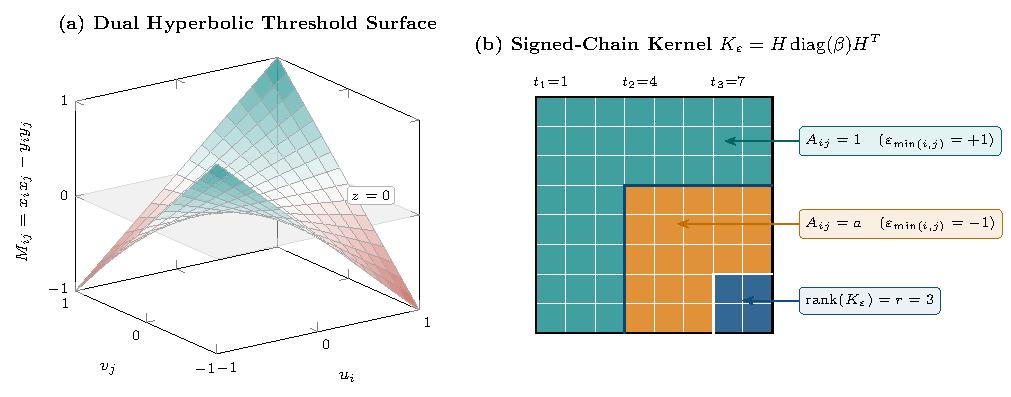
\includegraphics[width=0.92\linewidth]{figures/fig2.pdf}
\caption{\textbf{Dual variational formulation and signed-chain kernel decomposition.} (a) The dual hyperbolic threshold surface $M_{ij} = x_i x_j - y_i y_j$ intersected by the zero-threshold cutting plane $z = 0$, illustrating entrywise decoupling into $+1$ and $a$. (b) Step structure of the signed-chain kernel $K_\varepsilon = H \operatorname{diag}(\beta) H^T$ with $r = 3$ runs, showing the nested L-shaped suffix indicators $h_k h_k^T$ and start indices $t_1, t_2, t_3$ (Proposition~\ref{prop:signed-chain}).}\label{fig:dual-kernel}
\end{figure}

\section{Exact Analysis of the Rank-Two Family \texorpdfstring{$B_{n, k}(a)$}{B\_\{n,k\}(a)}}

For $1 \le k \le n-1$, let $e_S \in \{0, 1\}^n$ indicate $S = \{1, \dots, k\}$ and define
\begin{equation}\label{eq:def-Bnk}
B_{n, k}(a) = \begin{pmatrix} a J_k & J_{k, n-k} \\ J_{n-k, k} & J_{n-k} \end{pmatrix} = J_n - (1-a) e_S e_S^T.
\end{equation}

\begin{theorem}[Spectral Formula for $B_{n, k}(a)$ {\cite{fallat2012spread}}]\label{thm:exact-spectrum}
For $n \ge 2$, $-1 \le a < 1$, and $1 \le k \le n-1$, $\rank(B_{n, k}(a)) = 2$ with $n-2$ eigenvalues equal to $0$ and two nonzero eigenvalues $\lambda_+ > 0 > \lambda_-$ given by
\[
\lambda_\pm = \frac{n - k(1-a) \pm \sqrt{[n - k(1-a)]^2 + 4(1-a)k(n-k)}}{2}.
\]
Consequently,
\begin{equation}\label{eq:exact-spread}
s(B_{n, k}(a))^2 = n^2 + 2n(1-a)k - (1-a)(3+a)k^2.
\end{equation}
\end{theorem}
\begin{proof}
Compressing $B_{n, k}(a)$ onto the orthonormal basis $e_S/\sqrt{k}$, $e_{S^c}/\sqrt{n-k}$ of its column space yields the $2 \times 2$ matrix
\[
T_2 = \begin{pmatrix} ak & \sqrt{k(n-k)} \\ \sqrt{k(n-k)} & n-k \end{pmatrix},
\]
with $\tr(T_2) = n - k(1-a)$ and $\det(T_2) = (a-1)k(n-k) < 0$. Its discriminant is $(n - k(1-a))^2 + 4(1-a)k(n-k) = n^2 + 2n(1-a)k - (1-a)(3+a)k^2$, and the orthogonal complement of $\operatorname{span}\{e_S, e_{S^c}\}$ lies in $\ker(B_{n, k}(a))$.
\end{proof}

\begin{theorem}[Discrete Cluster Optimization {\cite{fallat2012spread}}]\label{thm:optimal-k}
Let $F(t) = n^2 + 2n(1-a)t - (1-a)(3+a)t^2$ for $t \in \R$ and $-1 \le a < 1$. Then:
\begin{enumerate}
    \item $F$ is strictly concave ($F''(t) = -2(1-a)(3+a) < 0$) with continuous maximizer $t^* = \frac{n}{3+a}$ and identity
    \begin{equation}\label{eq:F-vertex}
    F(t) = \frac{4n^2}{3+a} - (1-a)(3+a)\left(t - \frac{n}{3+a}\right)^2.
    \end{equation}
    \item Over integers $k \in \{1, \dots, n-1\}$, the maximum $M_n(a)^2 := \max_{1 \le k < n} F(k)$ is attained at a nearest integer $k^* = \operatorname{round}(n/(3+a))$ (when $n = 2$ and $a = 0$, $t^* = 2/3$ rounds to the unique valid integer $k^* = 1$).
\end{enumerate}
\end{theorem}

Table~\ref{tab:comparisons} summarizes exact agreement between \eqref{eq:exact-spread} and prior benchmarks.

\begin{table}[t]
\centering
\small
\caption{Agreement of the closed-form rank-two spread formula \eqref{eq:exact-spread} with certified benchmarks in the prior literature.}
\label{tab:comparisons}
\resizebox{\textwidth}{!}{%
\begin{tabular}{cccccc}
\toprule
$(n, a)$ & Reference & Optimal $k^*$ & Benchmark $s(A)$ & Formula $s(B_{n, k^*})$ & Agreement \\
\midrule
$n$ (even), $a=-1$ & Zhan \cite{zhan2005extremal} & $n/2$ & $\sqrt{2}\,n$ & $\sqrt{2}\,n$ & Exact \\
$n$ (odd), $a=-1$ & Zhan \cite{zhan2005extremal} & $(n-1)/2$ & $\sqrt{2n^2-1}$ & $\sqrt{2n^2-1}$ & Exact \\
$3 \mid n$, $a=0$ & Calkin et al.\ \cite{corless2025bohemian} & $n/3$ & $\frac{2\sqrt{3}}{3}n$ & $\frac{2\sqrt{3}}{3}n$ & Exact \\
$(8, 1/2)$ & Holden \cite{holden2026a} & $2$ & $\sqrt{73}$ & $\sqrt{73}$ & Exact \\
$(10, 0)$ & Holden \cite{holden2026a} & $3$ & $\sqrt{133}$ & $\sqrt{133}$ & Exact \\
$(11, 0)$ & Holden \cite{holden2026a} & $4$ & $\sqrt{161}$ & $\sqrt{161}$ & Exact \\
\bottomrule
\end{tabular}%
}
\end{table}

\begin{figure}[htbp]
\centering
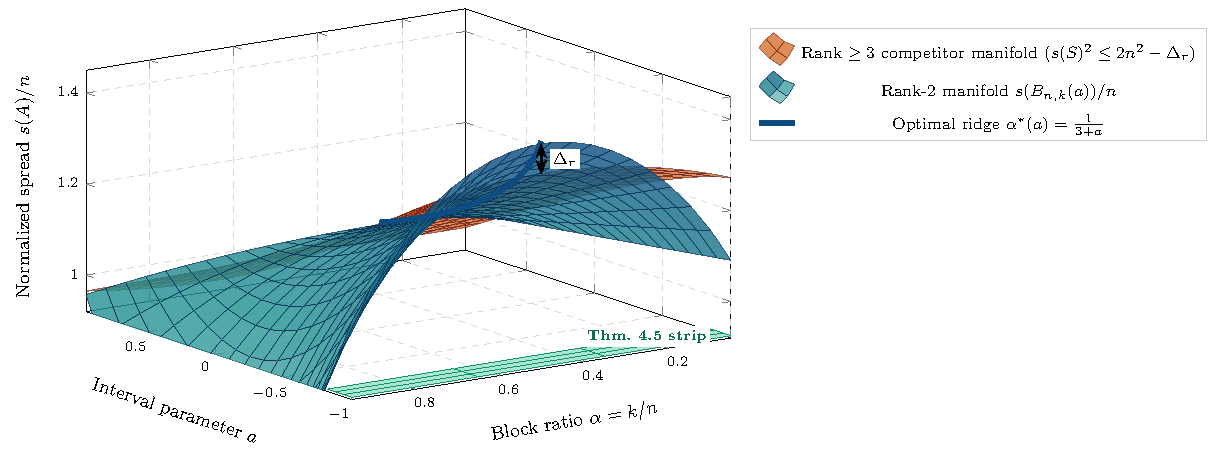
\includegraphics[width=0.88\linewidth]{figures/fig1.pdf}
\caption{\textbf{Normalized spectral spread manifold and universal spectral gap.} The upper surface (teal/navy) displays the normalized rank-two spread manifold $s(B_{n,k}(a))/n = \sqrt{1 + 2(1-a)\alpha - (1-a)(3+a)\alpha^2}$ as a function of the entry parameter $a \in [-1, 1)$ and block ratio $\alpha = k/n$. The dark ridge line marks the optimal continuous trajectory $\alpha^*(a) = \frac{1}{3+a}$ (Theorem~\ref{thm:optimal-k}). The lower surface (amber/crimson) illustrates the competitor manifold for matrices with $\operatorname{rank}(S) \ge 3$, separated by the universal secant spectral deficit $\Delta_r$ at the boundary $a = -1$ (Theorem~\ref{thm:all-runs-gap}). The floor strip (emerald) marks the boundary region covered by Theorem~\ref{thm:widened-strip}.}\label{fig:3d-manifold}
\end{figure}

\section{Rank-Three Sign Matrix Classification and Sharpened Boundary Strips}

Write any endpoint matrix $A \in \{a, 1\}^{n \times n}_{\text{sym}}$ in centered affine coordinates
\begin{equation}\label{eq:affine-centered}
A = \mu J_n + \rho S, \qquad \mu := \frac{1+a}{2},\quad \rho := \frac{1-a}{2} = 1 - \mu, \quad S \in \{-1, 1\}^{n \times n}_{\text{sym}}.
\end{equation}
In Appendix~\ref{app:centered-rank2}, following \cite{holden2026b}, we provide a self-contained proof that $s(A) \le M_n(a)$ for all $-1 \le a \le 0$ whenever $\rank(S) \le 2$. To bound matrices with $\rank(S) \ge 3$, we first classify all rank-three symmetric sign matrices completely.

\subsection{Complete Classification of Rank-Three Symmetric Sign Matrices}

\begin{lemma}[Classification and Exact Cubics of Rank-Three Sign Matrices]\label{lem:rank3-class}
Let $S \in \{-1, 1\}^{n \times n}$ ($n \ge 3$) be symmetric with $\rank(S) = 3$. Then there exist integers $p, q, r \ge 1$ with $p + q + r = n$, a sign $\xi \in \{-1, 1\}$, a permutation matrix $P$, and a diagonal signature $\Delta = \diag(\pm 1)$ such that $P^T S P = \xi \Delta B \Delta$, where $B$ takes one of two block forms:
\begin{enumerate}
    \item \textbf{Type I ($T_-$ blow-up):}
    \[
    B^-_{p,q,r} = \begin{pmatrix} J_p & J_{p,q} & J_{p,r} \\ J_{q,p} & -J_q & J_{q,r} \\ J_{r,p} & J_{r,q} & -J_r \end{pmatrix},
    \]
    whose three nonzero eigenvalues are the roots of
    \begin{equation}\label{eq:cubic-minus}
    P^-_{p,q,r}(\lambda) = \lambda^3 - (p - q - r)\lambda^2 - 2p(q+r)\lambda - 4pqr = 0.
    \end{equation}
    \item \textbf{Type II ($T_+$ blow-up):}
    \[
    B^+_{p,q,r} = \begin{pmatrix} J_p & J_{p,q} & J_{p,r} \\ J_{q,p} & J_q & -J_{q,r} \\ J_{r,p} & -J_{r,q} & J_r \end{pmatrix},
    \]
    whose three nonzero eigenvalues are the roots of
    \begin{equation}\label{eq:cubic-plus}
    P^+_{p,q,r}(\lambda) = \lambda^3 - n\lambda^2 + 4pqr = 0.
    \end{equation}
\end{enumerate}
\end{lemma}
\begin{proof}
Since $\rank(S) = 3$, the coefficient of $\lambda^{n-3}$ in $\det(\lambda I - S)$ is $-\lambda_1 \lambda_2 \lambda_3 \ne 0$, which equals minus the sum of all $3 \times 3$ principal minors of $S$. Hence $S$ has a nonsingular $3 \times 3$ principal submatrix $M \in \{-1, 1\}^{3 \times 3}$. Up to overall sign $\xi \in \{-1, 1\}$, permutation of the full index set $\{1, 2, 3\}$, and diagonal sign conjugation $\diag(1, M_{12}, M_{13}) M \diag(1, M_{12}, M_{13})$ (applied after diagonal-entry ordering so that row $1$ and column $1$ become $\one_3$ while the diagonal entries remain fixed), only two equivalence classes exist:
\begin{itemize}
    \item If all three diagonal entries of $M$ are equal (normalized via $\xi$ to $(1, 1, 1)$), then $M_{23} = 1$ yields singular $J_3$, while $M_{23} = -1$ yields
    \[
    T_+ = \begin{pmatrix} 1 & 1 & 1 \\ 1 & 1 & -1 \\ 1 & -1 & 1 \end{pmatrix}, \qquad \det(T_+) = -4.
    \]
    \item If the diagonal entries are not all equal, applying a global sign $\xi$ and a permutation of $\{1, 2, 3\}$ places the unique $+1$ diagonal entry at index~$1$, normalizing $\diag(M) = (1, -1, -1)$; conjugating by $\diag(1, M_{12}, M_{13})$ then leaves $(M_{22}, M_{33}) = (-1, -1)$ invariant and forces row and column~$1$ to be $\one_3$. Setting $M_{23} = -1$ repeats rows $2$ and $3$ (singular), whereas $M_{23} = 1$ yields
    \[
    T_- = \begin{pmatrix} 1 & 1 & 1 \\ 1 & -1 & 1 \\ 1 & 1 & -1 \end{pmatrix}, \qquad \det(T_-) = 4.
    \]
\end{itemize}
Reordering indices so $M$ occupies the leading $3 \times 3$ principal block and normalizing $M \in \{T_-, T_+\}$, let $b \in \{-1, 1\}^3$ denote the first three entries of any column $i \in \{1, \dots, n\}$. Since $\rank(S) = 3 = \rank(M)$, the Schur complement of $M$ in $S$ vanishes identically, forcing $S_{ii} = b^T M^{-1} b \in \{-1, 1\}$. Explicit inverses give
\begin{align*}
T_-^{-1} &= \frac{1}{2}\begin{pmatrix} 0 & 1 & 1 \\ 1 & -1 & 0 \\ 1 & 0 & -1 \end{pmatrix}
\implies b^T T_-^{-1} b = b_1(b_2 + b_3) - 1, \\
T_+^{-1} &= \frac{1}{2}\begin{pmatrix} 0 & 1 & 1 \\ 1 & 0 & -1 \\ 1 & -1 & 0 \end{pmatrix}
\implies b^T T_+^{-1} b = b_1(b_2 + b_3) - b_2 b_3.
\end{align*}
For $M = T_-$, choosing $b = \pm(-1, 1, 1)^T$ gives $-3 \notin \{-1, 1\}$, leaving only $\pm$ the three columns of $T_-$. For $M = T_+$, choosing $b = \pm(1, -1, -1)^T$ gives $-3 \notin \{-1, 1\}$, leaving only $\pm$ the three columns of $T_+$. Grouping columns by which column of $T_\pm$ they match up to sign (absorbing those column signs into $\Delta = \diag(\pm 1)$) produces $\Delta B^-_{p,q,r} \Delta$ or $\Delta B^+_{p,q,r} \Delta$ with $p, q, r \ge 1$ and $p + q + r = n$.

Compressing $B^\pm_{p,q,r}$ onto the orthonormal basis of its three block indicator vectors gives the $3 \times 3$ matrix $D_3^{1/2} T_\pm D_3^{1/2}$ with $D_3 = \diag(p, q, r)$, whose characteristic polynomials are directly computed as \eqref{eq:cubic-minus} and \eqref{eq:cubic-plus}.
\end{proof}

\subsection{Universal Rank \texorpdfstring{$\ge 3$}{>= 3} Spectral Gaps}

Set $\delta_* := 16 - 8\sqrt{2} \approx 4.6862915$.

\begin{theorem}[Universal Spectral Gaps for Rank $\ge 3$ Sign Matrices]\label{thm:rank3-gap}
Let $S \in \{-1, 1\}^{n \times n}$ be symmetric with $\rank(S) \ge 3$.
\begin{enumerate}
    \item For every $n \ge 4$,
    \begin{equation}\label{eq:rank3-gap-4}
    s(S)^2 < 2n^2 - 3.
    \end{equation}
    \item For every $n \ge 7$,
    \begin{equation}\label{eq:rank3-gap-7}
    s(S)^2 \le 2n^2 - \delta_* = 2n^2 - (16 - 8\sqrt{2}).
    \end{equation}
\end{enumerate}
\end{theorem}
\begin{proof}
We analyze $\rank(S) = 3$ and $\rank(S) \ge 4$ separately.

\medskip\noindent\textbf{Case 1: $\rank(S) = 3$, Type II ($T_+$ blow-up).}
By Lemma~\ref{lem:rank3-class}, up to sign $\xi$ the nonzero eigenvalues solve $P^+_{p,q,r}(\lambda) = \lambda^3 - n\lambda^2 + 4pqr = 0$. Since $P^+(0) = 4pqr > 0$, $P^+(1) = 4pqr - n + 1 \ge 4(n-2) - n + 1 = 3n - 7 > 0$ for $n \ge 4$, and at $\lambda = 2n/3$ AM-GM gives $P^+(2n/3) = 4pqr - \frac{4}{27}n^3 \le 0$, the three nonzero roots satisfy $\lambda_1 \ge \lambda_2 > 1 > 0 > \lambda_3$. Since $n \ge 4$, $\lambda_{\max}(S) = \lambda_1$ and $\lambda_{\min}(S) = \lambda_3$ (after $\xi = +1$), with $\lambda_1 + \lambda_2 + \lambda_3 = n$ and $\lambda_1^2 + \lambda_2^2 + \lambda_3^2 = n^2$. Hence
\begin{align*}
s(S)^2 &= (\lambda_1 - \lambda_3)^2 = 2(\lambda_1^2 + \lambda_3^2) - (\lambda_1 + \lambda_3)^2 \\
&= 2(n^2 - \lambda_2^2) - (n - \lambda_2)^2
= 2n^2 - \left[3\left(\lambda_2 - \frac{n}{3}\right)^2 + \frac{2}{3}n^2\right]
\le \frac{4}{3}n^2,
\end{align*}
which is strictly less than $2n^2 - 3$ for all $n \ge 4$ and strictly less than $2n^2 - \delta_*$ for all $n \ge 3$ (since $\frac{2}{3}n^2 \ge 6 > \delta_*$).

\medskip\noindent\textbf{Case 2: $\rank(S) = 3$, Type I ($T_-$ blow-up).}
Up to overall sign $\xi$, the nonzero eigenvalues solve $P^-_{p,q,r}(\lambda) = 0$ with $p, q, r \ge 1$ and $p + q + r = n \ge 4$. Put $w := q + r \ge 2$ and $\tau := p - w = \tr(B^-_{p,q,r}) \in \Z$. Direct evaluation gives $P^-_{p,q,r}(0) = -4pqr < 0$,
\[
P^-_{p,q,r}(-w) = -w^3 - (p-w)w^2 + 2pw^2 - 4pqr = p(q-r)^2 \ge 0,
\]
and
\[
P^-_{p,q,r}(-1) = (w - 1) - p(2q - 1)(2r - 1).
\]
If $q = r = 1$, then $p = n - 2 \ge 2$ yields $P^-_{p,1,1}(-1) = 1 - p < 0$; if $\max(q,r) \ge 2$, then $(2q-1)(2r-1) - (w - 1) = (2q-2)(2r-2) + w - 2 > 0$, so $P^-_{p,q,r}(-1) < 0$ in every case. Hence the roots satisfy $\lambda_3 \le -w \le \lambda_2 < -1 < 0 < \lambda_1$. Setting $\eta_2 := -\lambda_2 > 1$, from $\lambda_1 + \lambda_3 = \eta_2 + \tau$ and $\lambda_1^2 + \lambda_3^2 = n^2 - \eta_2^2$ we obtain
\begin{equation}\label{eq:rank3-exact-gap}
s(S)^2 = (\lambda_1 - \lambda_3)^2 = 2n^2 - \bigl[2\eta_2^2 + (\eta_2 + \tau)^2\bigr].
\end{equation}
For \emph{all $n \ge 4$}, we show $2\eta_2^2 + (\eta_2 + \tau)^2 > 3$:
\begin{itemize}
    \item $\tau \ge 0$: since $\eta_2 > 1$, $2\eta_2^2 + (\eta_2 + \tau)^2 \ge 3\eta_2^2 > 3$.
    \item $\tau = -2$: $2\eta_2^2 + (\eta_2 - 2)^2 - 3 = (\eta_2 - 1)(3\eta_2 - 1) > 0$.
    \item $\tau \le -3$: completing the square yields $2\eta_2^2 + (\eta_2 + \tau)^2 = 3(\eta_2 + \tau/3)^2 + \frac{2}{3}\tau^2 \ge \frac{2}{3}\tau^2 \ge 6 > 3$.
    \item $\tau = -1$: here $w = p + 1$, so $2p + 1 = n \ge 4 \implies p \ge 2$, and $(q-1)(r-1) \ge 0 \implies qr \ge w - 1 = p$. Evaluating at $\lambda = -4/3 \in (-w, -1)$ yields
    \[
    P^-_{p,q,r}\!\left(-\frac{4}{3}\right)
    = -\frac{16}{27} + \frac{8}{3}p(p+1) - 4pqr
    \le -\frac{16}{27} - \frac{4}{3}p(p - 2) \le -\frac{16}{27} < 0.
    \]
    Thus $\eta_2 > 4/3$, giving $2\eta_2^2 + (\eta_2 - 1)^2 > 2(4/3)^2 + (1/3)^2 = 11/3 > 3$.
\end{itemize}
Now suppose \emph{$n \ge 7$}. Completing the square gives $2\eta_2^2 + (\eta_2 + \tau)^2 \ge \frac{2}{3}\tau^2$; if $|\tau| \ge 3$, this is at least $6 > \delta_*$. If $\tau \ge 1$, since $\eta_2 > 1$ we obtain $2\eta_2^2 + (\eta_2 + \tau)^2 > 2(1)^2 + (2)^2 = 6 > \delta_*$. In the remaining cases $\tau \in \{0, -1, -2\}$, $2w = n - \tau \ge 7$ forces $w \ge 4$, and $qr \ge w - 1$ gives $-3pw + 4pqr \ge p(w - 4) \ge 0$. Defining $Q(\eta) := -P^-_{p,q,r}(-\eta) = \eta^3 + \tau \eta^2 - 2pw\eta + 4pqr$, we have $Q(w) = -p(q-r)^2 \le 0$ and
\[
Q\!\left(\frac{3}{2}\right) = \frac{27}{8} + \frac{9}{4}\tau - 3pw + 4pqr \ge \frac{27}{8} + \frac{9}{4}\tau + p(w - 4).
\]
If $\tau \in \{0, -1\}$, then $\frac{27}{8} + \frac{9}{4}\tau \ge \frac{9}{8} > 0$ and $p(w-4) \ge 0$; if $\tau = -2$, then $2p + 2 = n \ge 7$ forces $p \ge 3$ and $w = p + 2 \ge 5$, so $p(w - 4) \ge 3$ and $\frac{27}{8} - \frac{9}{2} + 3 = \frac{15}{8} > 0$. Thus $Q(3/2) > 0$ for all $\tau \in \{0, -1, -2\}$ whenever $n \ge 7$, forcing $\eta_2 > 3/2$. For each $\tau \in \{0, -1, -2\}$, define $\phi_\tau(\eta) := 2\eta^2 + (\eta + \tau)^2$. Its derivative is $\phi_\tau'(\eta) = 6\eta + 2\tau > 6(3/2) + 2(-2) = 5 > 0$ for all $\eta > 3/2$, so $\phi_\tau$ is strictly increasing on $(3/2, \infty)$. Therefore,
\[
2\eta_2^2 + (\eta_2 + \tau)^2 = \phi_\tau(\eta_2) > \phi_\tau\left(\frac{3}{2}\right) = \frac{9}{2} + \left(\frac{3}{2} + \tau\right)^2 \ge \frac{19}{4} = 4.75 > 16 - 8\sqrt{2} = \delta_*.
\]

\medskip\noindent\textbf{Case 3: $\rank(S) \ge 4$.}
Because $\rank(S) \ge 4$, $S$ contains a nonsingular $4 \times 4$ submatrix $T_4 \in \{-1, 1\}^{4 \times 4}$. Subtracting row~$1$ of $T_4$ from rows~$2, 3, 4$ leaves entries in $\{0, \pm 2\}$, so $8 \mid \det(T_4)$. Since $T_4$ is nonsingular, $\det(T_4^T T_4) = \det(T_4)^2 \ge 64$. Let $\sigma_1 \ge \sigma_2 \ge \sigma_3 \ge \sigma_4 > 0$ be the singular values of $T_4$, and set $A_0 = \sigma_1^2 + \sigma_2^2$ and $B_0 = \sigma_3^2 + \sigma_4^2$, so $A_0 + B_0 = \|T_4\|_F^2 = 16$ and $0 < B_0 \le 8 \le A_0$. By AM-GM on $(\sigma_1^2, \sigma_2^2)$ and $(\sigma_3^2, \sigma_4^2)$,
\[
64 \le \sigma_1^2 \sigma_2^2 \sigma_3^2 \sigma_4^2 \le \frac{A_0^2 B_0^2}{16}
\implies B_0(16 - B_0) \ge 32
\implies B_0^2 - 16 B_0 + 32 \le 0.
\]
Since $B_0 \le 8$, this forces
\begin{equation}\label{eq:sigma34}
\sigma_3(T_4)^2 + \sigma_4(T_4)^2 = B_0 \ge 8 - 4\sqrt{2}.
\end{equation}
Writing $S = \sum_{i=1}^n \lambda_i u_i u_i^T$ in an orthonormal eigenbasis and setting $X = \lambda_1 u_1 u_1^T + \lambda_n u_n u_n^T$ ($\rank(X) \le 2$), let $R_4$ be the $4 \times 4$ submatrix of $X$ at the positions of $T_4$; then $\rank(R_4) \le 2$. By the Eckart-Young-Mirsky theorem and \eqref{eq:sigma34},
\[
n^2 - (\lambda_1^2 + \lambda_n^2) = \sum_{i=2}^{n-1} \lambda_i^2 = \|S - X\|_F^2 \ge \|T_4 - R_4\|_F^2 \ge \sigma_3(T_4)^2 + \sigma_4(T_4)^2 \ge 8 - 4\sqrt{2}.
\]
Consequently, for every $n \ge 4$,
\[
s(S)^2 = (\lambda_1 - \lambda_n)^2 \le 2(\lambda_1^2 + \lambda_n^2) \le 2n^2 - (16 - 8\sqrt{2}) < 2n^2 - 3. \qedhere
\]
\end{proof}

\begin{theorem}[Sharp All-Runs Spectral Deficit for Signed-Threshold Matrices]\label{thm:all-runs-gap}
Let $S = D K_\varepsilon D$ with $D = \diag(d)$, $d \in \{-1, 1\}^n$, and $(K_\varepsilon)_{ij} = \varepsilon_{\min(i, j)}$ be a signed-threshold sign matrix. If $\varepsilon$ has at least $r \ge 2$ maximal constant-sign runs (so $\rank(S) \ge r$ by Proposition~\ref{prop:signed-chain}), then
\begin{equation}\label{eq:all-runs-gap}
s(S)^2 \le 2n^2 - \Delta_r, \qquad \Delta_r := 2r^2 - 4\csc^2\left(\frac{\pi}{2r}\right).
\end{equation}
The deficit $\Delta_r$ is the best constant independent of the dimension $n$: equality holds at $n = r$ for $S = T_r$, where $(T_r)_{ij} = (-1)^{\min(i, j) - 1}$. For $n > r$, the bound is in general strict; for example, for the balanced block blow-up of $T_r$ one has $s(S)^2 = 2n^2 - (n/r)^2 \Delta_r$, and for $r=3$, $n \ge 4$ the deficit is strictly improved by Theorem~\ref{thm:rank3-gap}. Moreover, as $r \to \infty$,
\begin{equation}
\Delta_r = \left(2 - \frac{16}{\pi^2}\right)r^2 - \frac{4}{3} + O(r^{-2}) \approx 0.37886\, r^2.
\end{equation}
\end{theorem}
\begin{proof}
Select the first index in each of the first $r$ constant-sign runs of $\varepsilon$, denoted $I = \{i_1 < i_2 < \dots < i_r\}$. Up to a global sign and diagonal signature conjugation $D[I]$, the $r \times r$ principal submatrix $S[I, I]$ is identical to $T_r \in \{-1, 1\}^{r \times r}$ with $(T_r)_{ij} = (-1)^{\min(i, j) - 1}$.

Let $L \in \{0, 1\}^{r \times r}$ be the unit lower triangular cumulative-sum matrix with $L_{ij} = \mathbf{1}_{i \ge j}$, and set $\beta_1 = 1$, $\beta_j = 2(-1)^{j-1}$ for $2 \le j \le r$. By Proposition~\ref{prop:signed-chain}, $T_r = L \diag(\beta_1, \dots, \beta_r) L^T$. Inverting both sides gives
\[
2 T_r^{-1} = 2 L^{-T} \diag(\beta_1^{-1}, \dots, \beta_r^{-1}) L^{-1}.
\]
Because $L^{-1}$ is the bidiagonal first-difference matrix ($1$ on the main diagonal, $-1$ on the subdiagonal), $2 T_r^{-1}$ is tridiagonal with main diagonal $(1, 0, \dots, 0, (-1)^{r-1})$ and alternating off-diagonal entries $\pm 1$. Conjugating by a diagonal sign signature yields a Jacobi tridiagonal matrix $J_r$ with all off-diagonal entries equal to $+1$.

For the trial eigenvector $v_j = \cos\bigl((j - \frac{1}{2})\theta\bigr)$, the interior tridiagonal recurrence gives $(J_r v)_j = 2\cos\theta\, v_j$. The left boundary condition at $j=1$ is satisfied identically, while the right boundary condition at $j=r$ enforces $\sin(r\theta) = 0$ when $r$ is odd, and $\cos(r\theta) = 0$ when $r$ is even. Hence the $r$ distinct eigenvalues of $J_r$ are $2\cos(k\pi / r)$ for $0 \le k < r$ ($r$ odd) and $2\cos\bigl((2k-1)\pi / (2r)\bigr)$ for $1 \le k \le r$ ($r$ even). None is zero, so the eigenvalues of $T_r$ are their reciprocals scaled by $2$:
\[
\operatorname{spec}(T_r) =
\begin{cases}
\{\sec(k\pi / r) : 0 \le k < r\} & \text{if } r \text{ is odd}, \\
\{\sec\bigl((2k-1)\pi / (2r)\bigr) : 1 \le k \le r\} & \text{if } r \text{ is even}.
\end{cases}
\]
Thus $\lambda_{\max}(T_r) = -\lambda_{\min}(T_r) = c_r := \csc\bigl(\frac{\pi}{2r}\bigr)$. Since $\|T_r\|_F^2 = r^2$, the best rank-two Frobenius residual of $T_r$ is precisely $q_r = r^2 - 2c_r^2$.

For the full matrix $S$, let $X = \lambda_{\max}(S) u u^T + \lambda_{\min}(S) v v^T$ with orthonormal extremal eigenvectors, so $\rank(X) \le 2$. By the Eckart-Young-Mirsky theorem on the principal submatrix $I$,
\[
n^2 - \lambda_{\max}(S)^2 - \lambda_{\min}(S)^2 = \|S - X\|_F^2 \ge \|S[I, I] - X[I, I]\|_F^2 \ge q_r.
\]
Consequently,
\[
s(S)^2 = (\lambda_{\max} - \lambda_{\min})^2 \le 2(\lambda_{\max}^2 + \lambda_{\min}^2) \le 2(n^2 - q_r) = 2n^2 - \Delta_r.
\]
For $S = T_r$ at $n = r$, the extremal eigenvalues are $\pm c_r$, so $s(T_r)^2 = 4c_r^2 = 2r^2 - \Delta_r$, attaining equality and proving that $\Delta_r$ is the optimal dimension-free constant deficit. Expanding $\sin(\frac{\pi}{2r}) = \frac{\pi}{2r}(1 - \frac{\pi^2}{24 r^2} + O(r^{-4}))$ yields the asymptotic formula.
\end{proof}

\begin{remark}[Hierarchy of Deficits and Cautions]\label{rem:all-runs-hierarchy}
Evaluating \eqref{eq:all-runs-gap} yields $\Delta_3 = 2$, $\Delta_4 = 16 - 8\sqrt{2} \approx 4.6863$ (recovering $\delta_*$), $\Delta_5 = 26 - 8\sqrt{5} \approx 8.1115$, and $\Delta_6 = 40 - 16\sqrt{3} \approx 12.2872$. We emphasize two distinctions:
\begin{enumerate}
    \item For $r=3$, the universal cubic analysis of Theorem~\ref{thm:rank3-gap} gives $s(S)^2 < 2n^2 - 3$ for all $n \ge 4$ (and $2n^2 - \delta_*$ for $n \ge 7$), which is sharper than $\Delta_3 = 2$ because Theorem~\ref{thm:rank3-gap} exploits the entire $n$-dimensional blow-up rather than restricting to $T_3$.
    \item Theorem~\ref{thm:all-runs-gap} bounds the centered sign matrix $S$, not the full affine matrix $A = \mu J_n + \rho S$. For $A$, subadditivity gives $s(A) \le \mu n + \rho \sqrt{2n^2 - \Delta_r}$. Because $A = \mu \one \one^T + \rho S$ with $\rank(\one \one^T) = 1$, $\rank(S) = 2$ only guarantees $\rank(A) \le 3$, and $\rank(A) = 3$ can occur whenever $\one \notin \operatorname{range}(S)$ (as analyzed in Appendix~\ref{app:centered-rank2}); closing the gap between $\rank(S)$ and $\rank(A)$ remains the central open frontier for $a > 0$.
\end{enumerate}
\end{remark}

\subsection{Sharpened Unrestricted All-Dimensions Boundary Strips}

\begin{theorem}[Sharpened Unrestricted Boundary Strips]\label{thm:widened-strip}
For any integer $n \ge 4$ and real $\delta \in (0, 2n^2)$ (evaluated specifically at $\delta \in \{3, 16 - 8\sqrt{2}\}$), set $\epsilon = n \bmod 2$, $k = \lfloor n/2 \rfloor = (n - \epsilon)/2$, $L_n(\delta) = \sqrt{2n^2 - \delta}$, and
\[
C_\epsilon(n; \delta) =
\begin{cases}
    2n L_n(\delta) - 2n^2 + \delta & \text{if } \epsilon = 0 \text{ ($n$ even)}, \\
    2n L_n(\delta) - 2n^2 - 2n + \delta + 1 & \text{if } \epsilon = 1 \text{ ($n$ odd)}.
\end{cases}
\]
Recall $\mu = \frac{1+a}{2}$, $\rho = \frac{1-a}{2} = 1 - \mu$, and $\delta_* = 16 - 8\sqrt{2}$. Then $B_{n, \lfloor n/2 \rfloor}(a)$ attains $\max_{A \in \mathcal{S}_n[a, 1]} s(A)$ (equaling $M_n(a)$) in both of the following regimes:
\begin{enumerate}
    \item \textbf{All $n \ge 4$ ($\delta = 3$):} whenever
    \begin{equation}\label{eq:sharp-strip-4}
    -1 \le a \le -1 + \frac{2(3 - \epsilon)}{C_\epsilon(n; 3)},
    \end{equation}
    which strictly contains the unified strip
    \begin{equation}\label{eq:unified-strip-4}
    -1 \le a \le -1 + \frac{2(1 + \sqrt{2})}{n^2} \qquad (\forall n \ge 4),
    \end{equation}
    doubling the unified strip of \cite{holden2026b}.
    \item \textbf{Sharpened regime for $n \ge 7$ ($\delta = \delta_* = 16 - 8\sqrt{2}$):} whenever
    \begin{equation}\label{eq:sharp-strip-7}
    -1 \le a \le -1 + \frac{2(\delta_* - \epsilon)}{C_\epsilon(n; \delta_*)},
    \end{equation}
    which strictly contains the unified strip
    \begin{equation}\label{eq:unified-strip-7}
    -1 \le a \le -1 + \frac{7\sqrt{2} - 1}{n^2} \approx -1 + \frac{8.8995}{n^2} \qquad (\forall n \ge 7),
    \end{equation}
    and for even $n \ge 8$ achieves the asymptotic upper bound $-1 + \frac{8\sqrt{2}}{n^2} \approx -1 + \frac{11.3137}{n^2}$. Since Calkin et al.\ \cite{corless2025bohemian} already proved SP-08 for $2 \le n \le 7$, this resolves new open parameter intervals for all $n \ge 8$.
\end{enumerate}
\end{theorem}
\begin{proof}
Write an endpoint matrix as $A = \mu J_n + \rho S$ with $S \in \{-1, 1\}^{n \times n}_{\text{sym}}$ (Proposition~\ref{prop:convexity}). Let $(\delta, n_0) \in \{(3, 4), (\delta_*, 7)\}$ and assume $n \ge n_0$ with $\mu \le \mu_{\text{sharp}} := (\delta - \epsilon)/C_\epsilon(n; \delta)$. First observe that for $n^2 > \frac{\delta}{4(\sqrt{2}-1)}$ (which holds for all $n \ge 2$ since $\frac{\delta_*}{4(\sqrt{2}-1)} = 2\sqrt{2} < 4$), squaring both sides verifies
\begin{equation}\label{eq:sqrt-lower}
2n L_n(\delta) - 2n^2 > 2(\sqrt{2} - 1)n^2 - \delta
\iff 4n^2(2n^2 - \delta) > (2\sqrt{2}n^2 - \delta)^2
\iff 4(\sqrt{2} - 1)\delta n^2 > \delta^2.
\end{equation}
We deduce $n\mu_{\text{sharp}} < 1$ separately for each parity:
\begin{itemize}
    \item If $\epsilon = 0$ ($n$ even), \eqref{eq:sqrt-lower} implies $C_0(n; \delta) > 2(\sqrt{2} - 1)n^2$, so $n\mu_{\text{sharp}} < \frac{\delta}{2(\sqrt{2}-1)n} \le \frac{3}{8(\sqrt{2}-1)} < 0.91 < 1$ when $\delta = 3, n \ge 4$, and $n\mu_{\text{sharp}} < \frac{\delta_*}{16(\sqrt{2}-1)} = \frac{\sqrt{2}}{2} < 0.71 < 1$ when $\delta = \delta_*, n \ge 8$.
    \item If $\epsilon = 1$ ($n$ odd), \eqref{eq:sqrt-lower} implies $C_1(n; \delta) > 2(\sqrt{2} - 1)n^2 - 2n + 1$. When $\delta = 3, n \ge 5$, $2(\sqrt{2}-1)n^2 - 4n + 1 > 0$, so $(\delta - 1)n = 2n < C_1(n; 3)$. When $\delta = \delta_*, n \ge 7$, $2(\sqrt{2}-1)n - (\delta_* + 1) > 0.11 > 0$, so $(\delta_* - 1)n < 2(\sqrt{2}-1)n^2 - 2n + 1 < C_1(n; \delta_*)$.
\end{itemize}
In all cases $n\mu < 1$, which implies $\mu < 1/4$ (so $a = -1 + 2\mu < 0$) and
\[
0 < \frac{n}{2} - \frac{n}{3 + a} = \frac{n\mu}{2(1+\mu)} < \frac{n\mu}{2} < \frac{1}{2}.
\]
Hence $k = \lfloor n/2 \rfloor$ is within $1/2$ of $n/(3+a)$ and attains $M_n(a)$ by Theorem~\ref{thm:optimal-k}.

Now if $\rank(S) \le 2$, since $a \le 0$, Theorem~\ref{thm:centered-rank2} (proved in Appendix~\ref{app:centered-rank2}) gives $s(A) \le M_n(a) = s(B_{n,k}(a))$. If $\rank(S) \ge 3$, subadditivity and Theorem~\ref{thm:rank3-gap} give $s(A) \le \mu n + \rho L_n(\delta)$. Meanwhile, substituting $k = (n-\epsilon)/2$ and $1 - a = 2\rho$ into \eqref{eq:exact-spread} yields
\[
s(B_{n, k}(a))^2 = n^2 + \rho^2(n - \epsilon)^2 + 2\rho\epsilon(n - \epsilon).
\]
Since $\rho = 1 - \mu$ and $L_n(\delta)^2 = 2n^2 - \delta$, expanding the difference gives the identity
\begin{equation}\label{eq:strip-comparison}
\frac{s(B_{n, k}(a))^2 - (\mu n + \rho L_n(\delta))^2}{\rho} = (\delta - \epsilon) - \mu\, C_\epsilon(n; \delta).
\end{equation}
Thus \eqref{eq:sharp-strip-4} and \eqref{eq:sharp-strip-7} imply $s(B_{n,k}(a)) \ge \mu n + \rho L_n(\delta) \ge s(A)$.

Finally, since $L_n(\delta) < \sqrt{2}n$:
\begin{itemize}
    \item For $\delta = 3$: $C_1(n; 3) < 2(\sqrt{2}-1)n^2 - 2n + 4 < 2(\sqrt{2}-1)n^2$ ($n \ge 5$) and $C_0(n; 3) < 2(\sqrt{2}-1)n^2 + 3 < 3(\sqrt{2}-1)n^2$ ($n \ge 4$), so $\mu \le \frac{1+\sqrt{2}}{n^2} = \frac{1}{(\sqrt{2}-1)n^2}$ implies $\mu \le \frac{3 - \epsilon}{C_\epsilon(n; 3)}$, yielding \eqref{eq:unified-strip-4}.
    \item For $\delta = \delta_*$ and $n \ge 7$: for odd $n \ge 7$, $-2n + \delta_* + 1 \le -14 + 5.69 < 0$, so $C_1(n; \delta_*) < 2(\sqrt{2}-1)n^2$, giving $\frac{\delta_* - 1}{C_1(n; \delta_*)} > \frac{15 - 8\sqrt{2}}{2(\sqrt{2}-1)n^2} = \frac{7\sqrt{2} - 1}{2n^2}$. For even $n \ge 8$, $C_0(n; \delta_*) < \bigl(2(\sqrt{2}-1) + \frac{\delta_*}{64}\bigr)n^2$, giving $\frac{\delta_*}{C_0(n; \delta_*)} > \frac{5.19}{n^2} > \frac{7\sqrt{2}-1}{2n^2} \approx \frac{4.4497}{n^2}$. Hence $\mu \le \frac{7\sqrt{2}-1}{2n^2}$, i.e., \eqref{eq:unified-strip-7}, holds for every $n \ge 7$, and for even $n \to \infty$, $\frac{2\delta_*}{C_0(n; \delta_*)} \sim \frac{\delta_*}{(\sqrt{2}-1)n^2} = \frac{8\sqrt{2}}{n^2}$. \qedhere
\end{itemize}
\end{proof}

\begin{remark}[Symmetry and Non-Uniqueness]\label{rem:symmetry}
Theorem~\ref{thm:widened-strip} asserts that $B_{n, \lfloor n/2 \rfloor}(a)$ attains the global maximum spread on $\mathcal{S}_n[a, 1]$, rather than strict uniqueness up to permutation similarity. Specifically, at $a = -1$, conjugating $B_{n, k}(-1)$ by $\diag(\one_k, -\one_{n-k})$ or taking $-B_{n, k}(-1)$ produces matrices with identical spectrum and spread that are not permutation-similar to $B_{n, k}(-1)$; for odd $n$ at $a = -1$, $B_{n, (n-1)/2}(-1)$ and $B_{n, (n+1)/2}(-1)$ have identical spread under this negation symmetry. Moreover, uniqueness among matrices with $\rank(S) \le 2$ relies on the strict comparison bounds of Theorem~\ref{thm:centered-rank2}.
\end{remark}

\section{Frobenius-Tail Identity and Exact Finite Certificates for \texorpdfstring{$n \in \{8, 9\}$}{n in \{8, 9\}}}

\subsection{Exact Frobenius-Tail Barrier Identity}

\begin{proposition}[Exact Frobenius-Tail Spread Identity]\label{prop:tail-identity}
Let $A \in \mathcal{S}_n$ have eigenvalues $\lambda_1 \ge \lambda_2 \ge \cdots \ge \lambda_n$, and define the residual interior trace and energy
\[
T_{\mathrm{int}} := \sum_{i=2}^{n-1} \lambda_i, \qquad Q_{\mathrm{int}} := \sum_{i=2}^{n-1} \lambda_i^2.
\]
Then:
\begin{enumerate}
    \item In general,
    \begin{equation}\label{eq:tail-general}
    s(A)^2 = 2\bigl(\|A\|_F^2 - Q_{\mathrm{int}}\bigr) - \bigl(\tr(A) - T_{\mathrm{int}}\bigr)^2.
    \end{equation}
    \item If $A = J_n - \delta H$ is an endpoint matrix with $\delta = 1 - a$, $H \in \{0, 1\}^{n \times n}_{\mathrm{sym}}$, $d_H = \tr(H)$, $m_H = \|H\|_F^2$, and effective defect $\tilde{d}_H := d_H + T_{\mathrm{int}}/\delta$, then
    \begin{equation}\label{eq:tail-endpoint}
    s(A)^2 = F(\tilde{d}_H) - 2(1 - a^2)(m_H - \tilde{d}_H^2) - 2Q_{\mathrm{int}},
    \end{equation}
    where $F(t) = n^2 + 2n\delta t - \delta(4 - \delta)t^2$ is the quadratic spread function \eqref{eq:exact-spread}.
\end{enumerate}
\end{proposition}
\begin{proof}
Since $\|A\|_F^2 = \lambda_1^2 + \lambda_n^2 + Q_{\mathrm{int}}$ and $\tr(A) = \lambda_1 + \lambda_n + T_{\mathrm{int}}$,
\[
s(A)^2 = (\lambda_1 - \lambda_n)^2 = 2(\lambda_1^2 + \lambda_n^2) - (\lambda_1 + \lambda_n)^2 = 2\bigl(\|A\|_F^2 - Q_{\mathrm{int}}\bigr) - \bigl(\tr(A) - T_{\mathrm{int}}\bigr)^2,
\]
proving \eqref{eq:tail-general}. For $A = J_n - \delta H$ with $H \in \{0,1\}^{n\times n}_{\mathrm{sym}}$, every entry of $A$ is $1$ (if $H_{ij} = 0$) or $1 - \delta$ (if $H_{ij} = 1$), so
\[
\tr(A) = n - \delta d_H, \qquad \|A\|_F^2 = (n^2 - m_H) + (1 - \delta)^2 m_H = n^2 - \delta(2 - \delta)m_H.
\]
Substituting these into \eqref{eq:tail-general} together with $T_{\mathrm{int}} = \delta(\tilde{d}_H - d_H)$ gives $\tr(A) - T_{\mathrm{int}} = n - \delta \tilde{d}_H$ and
\begin{align*}
s(A)^2 &= 2\bigl(n^2 - \delta(2 - \delta)m_H - Q_{\mathrm{int}}\bigr) - (n - \delta \tilde{d}_H)^2 \\
&= n^2 + 2n\delta \tilde{d}_H - \delta^2 \tilde{d}_H^2 - 2\delta(2 - \delta)m_H - 2Q_{\mathrm{int}} \\
&= \bigl[n^2 + 2n\delta \tilde{d}_H - \delta(4 - \delta)\tilde{d}_H^2\bigr] - 2\delta(2 - \delta)(m_H - \tilde{d}_H^2) - 2Q_{\mathrm{int}},
\end{align*}
which is \eqref{eq:tail-endpoint} since $\delta(2-\delta) = (1-a)(1+a) = 1 - a^2$.
\end{proof}

\begin{remark}[Behavior at $a = -1$ vs.\ General $a \in (-1, 1)$]
When $a = -1$, the coefficient $1 - a^2$ vanishes and \eqref{eq:tail-endpoint} simplifies to
\[
s(A)^2 = 2n^2 - (n - 2\tilde{d}_H)^2 - 2Q_{\mathrm{int}} \le 2n^2,
\]
which directly yields Zhan's even-$n$ bound $\sqrt{2}\,n$ (though Zhan's sharper odd-$n$ bound $\sqrt{2n^2 - 1}$ requires an additional integrality/parity argument to establish $(n - 2\tilde{d}_H)^2 + 2Q_{\mathrm{int}} \ge 1$). For general $a \in (-1, 1)$, $1 - a^2 > 0$, and $T_{\mathrm{int}}/\delta$ can shift $\tilde{d}_H = d_H + T_{\mathrm{int}}/\delta$ so that $m_H - \tilde{d}_H^2 < 0$, making $-2(1-a^2)(m_H - \tilde{d}_H^2) > 0$. Thus naive Frobenius-energy dominance fails unless $m_H - \tilde{d}_H^2$, $T_{\mathrm{int}}$, and $Q_{\mathrm{int}}$ are controlled simultaneously.
\end{remark}

\subsection{Five Newly Certified Finite Cases}

To establish exact optimality for rational parameters $(n, a) = (n, \ell / b)$ with coprime integers $\ell < b$, $b > 0$, we scale $[a, 1]$ by $b$ to $[\ell, b]$ (scaling all spreads by $b$). Every signed-threshold candidate $A \in \{\ell, b\}^{n \times n}_{\text{sym}}$ generated by Theorem~\ref{thm:signed-threshold} has monic integer characteristic polynomial $p(z) = \det(zI - A) = z^n + c_1 z^{n-1} + \cdots + c_n \in \Z[z]$. Following \cite{holden2026a}:

\begin{lemma}[Rational Shifted-Polynomial Enclosure]\label{lem:poly-shift}
Let $p(z) = z^n + c_1 z^{n-1} + \cdots + c_n \in \Z[z]$ be monic and let $u, D \in \Z$ with $D > 0$.
\begin{enumerate}
    \item If all coefficients of $D^n p((z+u)/D) \in \Z[z]$ are nonnegative, then $p$ has no real root exceeding $u/D$.
    \item Consequently, if $D^n p((z + u_+)/D)$ and $D^n p_-((z + u_-)/D)$ (where $p_-(z) = (-1)^n p(-z)$) both have only nonnegative coefficients and $0 \le u_+ + u_- \le D M$, then $\lambda_{\max}(A) - \lambda_{\min}(A) \le (u_+ + u_-)/D \le M$.
\end{enumerate}
\end{lemma}
\begin{proof}
Since $p$ is monic and $D > 0$, $D^n p((z+u)/D)$ has leading coefficient $1$. Nonnegativity of all coefficients makes $D^n p((z+u)/D) > 0$ for every $z > 0$, excluding any root above $u/D$. Applying the same criterion to $p_-$ bounds $-\lambda_{\min}(A) \le u_-/D$.
\end{proof}

All characteristic polynomials over the $2^{2n-1}$ patterns in Theorem~\ref{thm:signed-threshold} are computed in exact \texttt{int64} Newton trace-power arithmetic with checked overflow bound $n 2^n (n \max(|\ell|, |b|))^n \le 9.14 \times 10^{14} < 2^{63}$, cross-checked per batch against an independent arbitrary-precision Python integer Faddeev-LeVerrier evaluator. Distinct polynomials partition cleanly by their degree/zero-root structure:
\begin{itemize}
    \item \textbf{Rank-1 ($c_2 = \dots = c_n = 0$, $c_1 \ne 0$):} exactly $2$ polynomials in each case ($s(A) = |c_1|$);
    \item \textbf{Indefinite rank-2 ($c_3 = \dots = c_n = 0$, $c_2 < 0$):} two nonzero roots of opposite sign, certified directly by discriminant $c_1^2 - 4c_2 \le M^2$;
    \item \textbf{Definite rank-2 ($c_3 = \dots = c_n = 0$, $c_2 > 0$):} two nonzero roots of the same sign together with $0 \in \operatorname{spec}(A)$ (since $n \ge 3$), giving $s(A) = (|c_1| + \sqrt{c_1^2 - 4c_2})/2 < |c_1| \le n$. Since $M_n(a)^2 \ge s(B_{n, 1}(a))^2 = n^2 + (1-a)(2n - 3 - a) > n^2$ for all $-1 \le a < 1$, we have $|c_1| < M_n(a)$ unconditionally;
    \item \textbf{Rank $\ge 3$ ($c_3, \dots, c_n$ not all zero):} certified via exact integer Taylor-shift positivity tests (Lemma~\ref{lem:poly-shift}), where floating-point eigenvalues only suggest candidate bounds $(u_+, u_-, D)$. Moreover, all rank-1 and definite rank-2 polynomials are simultaneously certified via Lemma~\ref{lem:poly-shift}.
\end{itemize}

\begin{theorem}[Five Newly Certified Finite Cases]\label{thm:new-finite}
Over the continuous entry box $\mathcal{S}_n[a, 1]$, Conjecture~\ref{conj:fx} holds for the five previously open pairs in Table~\ref{tab:new-certs} (via Theorem~\ref{thm:signed-threshold}), with maximal spread attained by $B_{n, k^*}(a)$ at the stated cluster size $k^*$.
\end{theorem}

\begin{table}[t]
\centering
\small
\caption{Summary of the five newly certified exact finite cases beyond Calkin et al.\ \cite{corless2025bohemian} and Holden \cite{holden2026a}. Polynomials are partitioned into rank-1 ($2$ in each case), rank-2 (shown as indefinite $c_2 < 0$ / total $c_2 \ne 0$ with two nonzero roots), and rank $\ge 3$ certified by Lemma~\ref{lem:poly-shift}. Note: The ``Distinct'' column counts distinct characteristic polynomial coefficient vectors at that specific node $a_0$ (which vary due to coincidence of integer values at different points), whereas the $5{,}643$ figure in Theorem~\ref{thm:complete-n8} represents the total number of algebraically distinct bivariate characteristic pencils over all non-two-block patterns.}
\label{tab:new-certs}
\resizebox{\textwidth}{!}{%
\begin{tabular}{ccccccccc}
\toprule
$(n, a)$ & $\{\ell, b\}$ & Patterns ($2^{2n-1}$) & Distinct & Rank-2 (Indef./Total) & Enclosures ($r{\ge}3$/All) & Failures & $k^*$ & Max Spread $s(A)$ \\
\midrule
$(8, -1/2)$ & $\{-1, 2\}$ & $32{,}768$  & $5{,}629$  & $30 / 34$ & $5{,}593 / 5{,}599$   & $0$ & $3$ & $\frac{\sqrt{409}}{2} \approx 10.111874$ \\
$(8, -1/3)$ & $\{-1, 3\}$ & $32{,}768$  & $5{,}641$  & $18 / 22$ & $5{,}617 / 5{,}623$   & $0$ & $3$ & $4\sqrt{6} \approx 9.797959$ \\
$(8, 1/3)$  & $\{1, 3\}$  & $32{,}768$  & $5{,}647$  & $11 / 22$ & $5{,}623 / 5{,}636$   & $0$ & $2$ & $\frac{4\sqrt{43}}{3} \approx 8.743251$ \\
$(9, 1/2)$  & $\{1, 2\}$  & $131{,}072$ & $19{,}138$ & $12 / 24$ & $19{,}112 / 19{,}126$ & $0$ & $3$ & $\frac{3\sqrt{41}}{2} \approx 9.604686$ \\
$(9, -1/2)$ & $\{-1, 2\}$ & $131{,}072$ & $19{,}118$ & $36 / 40$ & $19{,}076 / 19{,}082$ & $0$ & $4$ & $\sqrt{129} \approx 11.357817$ \\
\bottomrule
\end{tabular}%
}
\end{table}

\begin{theorem}[Certified Nonzero Open Neighborhoods in $a$]\label{thm:open-intervals}
For each parameter pair $(n, a_0)$ in Table~\ref{tab:new-certs}, let $M_0 = M_n(a_0)$ and let $U < M_0$ be the certified rational upper bound on all non-$B$-shaped signed-threshold candidates at $a_0$. Setting $L_8 = \sqrt{85} = \max_{H \in \mathcal{S}_8[0, 1]} s(H)$ and $L_9 = 6\sqrt{3} = \max_{H \in \mathcal{S}_9[0, 1]} s(H)$ (from \cite{corless2025bohemian}), Conjecture~\ref{conj:fx} holds over the continuous entry box $\mathcal{S}_n[a, 1]$ for every real $a \in (a_0 - r, a_0 + r)$, where
\begin{equation}
r = \frac{M_0 - U}{2 L_n} > 0.
\end{equation}
In particular, the Fallat-Xing conjecture holds unconditionally across the five open intervals (certified by \texttt{verify\_sp08\_intervals.py}):
\begin{itemize}
    \item $n=8$, around $-1/2$: $a \in \bigl(-\frac{1}{2} - \frac{\sqrt{409}-20}{4\sqrt{85}},\, -\frac{1}{2} + \frac{\sqrt{409}-20}{4\sqrt{85}}\bigr) \approx (-0.506067, -0.493933)$;
    \item $n=8$, around $-1/3$: $a \in \bigl(-\frac{1}{3} - \frac{40\sqrt{6}-97}{20\sqrt{85}},\, -\frac{1}{3} + \frac{40\sqrt{6}-97}{20\sqrt{85}}\bigr) \approx (-0.338646, -0.328021)$;
    \item $n=8$, around $1/3$: $a \in \bigl(\frac{1}{3} - \frac{400\sqrt{43}-2619}{600\sqrt{85}},\, \frac{1}{3} + \frac{400\sqrt{43}-2619}{600\sqrt{85}}\bigr) \approx (0.332615, 0.334052)$;
    \item $n=9$, around $1/2$: with certified bound $U = 959/100$, $a \in \bigl(\frac{1}{2} - \frac{150\sqrt{41}-959}{1200\sqrt{3}},\, \frac{1}{2} + \frac{150\sqrt{41}-959}{1200\sqrt{3}}\bigr) \approx (0.499293, 0.500707)$;
    \item $n=9$, around $-1/2$: $a \in \bigl(-\frac{1}{2} - \frac{4\sqrt{129}-45}{48\sqrt{3}},\, -\frac{1}{2} + \frac{4\sqrt{129}-45}{48\sqrt{3}}\bigr) \approx (-0.505187, -0.494813)$.
\end{itemize}
\end{theorem}
\begin{proof}
Every signed-threshold matrix has the form $A(a) = J_n - (1-a)H$ for a fixed symmetric matrix $H \in \{0, 1\}^{n \times n}$. By subadditivity of the spectral spread,
\[
|s(A(a)) - s(A(a_0))| \le s\bigl((a - a_0)H\bigr) = |a - a_0| s(H) \le L_n |a - a_0|.
\]
For any non-$B$-shaped pattern $A(a)$, the exact rational shifted-polynomial certificates in \texttt{verify\_sp08\_intervals.py} prove $s(A(a_0)) \le U$, so $s(A(a)) \le U + L_n |a - a_0|$. Meanwhile, the maximal $B$-shaped candidate satisfies $M_n(a) \ge M_0 - L_n |a - a_0|$. Thus, for any $a$ satisfying $|a - a_0| < r = (M_0 - U)/(2 L_n)$, we have
\[
M_n(a) \ge M_0 - L_n |a - a_0| > U + L_n |a - a_0| \ge s(A(a)),
\]
proving that no non-$B$-shaped matrix can achieve the maximal spread on $(a_0 - r, a_0 + r)$.
\end{proof}

\subsection{Certified One-Sided Endpoint Neighborhood at \texorpdfstring{$a \to 1^-$}{a -> 1-} for \texorpdfstring{$n=8$}{n=8}}

While Theorem~\ref{thm:open-intervals} certifies open intervals around isolated points, such fixed-radius neighborhoods cannot reach the boundary $a \to 1^-$, because the spectral gap $M_n(a) - s(A(a))$ between the optimal rank-two candidate and non-$B$ candidates vanishes as $a \to 1^-$. In this section, we establish a dedicated analytic and exact integer certificate establishing Conjecture~\ref{conj:fx} throughout a full one-sided interval adjoining $a = 1$ in dimension $8$.

\begin{lemma}[Quadratic Remainder Bound for Leading-Order Perturbation]\label{lem:rem}
Let $H \in \{0, 1\}^{8 \times 8}_{\rm sym}$, $0 < \delta < 1/2$, $A_\delta = J_8 - \delta H$, $u = \frac{1}{\sqrt{8}}\one$, $h = u^T H u = \frac{1}{8}\one^T H \one$, $b = P H u$, and $C = (P H P)|_{u^\perp}$. Then
\begin{equation}\label{eq:rem-bound}
s(A_\delta) \le 8 + \delta c_1(H) + \frac{16\delta^2}{1 - 2\delta}, \qquad c_1(H) := \lambda_{\max}(C) - h.
\end{equation}
\end{lemma}
\begin{proof}
In an orthonormal basis extending $u$, write $A_\delta = \begin{pmatrix} \alpha & w^T \\ w & D \end{pmatrix}$ with $\alpha = 8 - \delta h \ge 8(1 - \delta)$, $w = -\delta b$, $\|w\|_2 \le 8\delta$, $D = -\delta C$, and $\|D\|_2 \le 8\delta$.
For the upper eigenvalue $\lambda_1 = \lambda_{\max}(A_\delta) \ge \alpha > \lambda_{\max}(D)$, the secular equation gives
\[
\lambda_1 - \alpha = w^T (\lambda_1 I - D)^{-1} w \le \frac{\|w\|_2^2}{\alpha - \lambda_{\max}(D)} \le \frac{64\delta^2}{8 - 16\delta} = \frac{8\delta^2}{1 - 2\delta}.
\]
For the lower eigenvalue $\lambda_8 = \lambda_{\min}(A_\delta) \le \lambda_{\min}(D) \le 8\delta < \alpha$, let $(t, y)$ be a normalized eigenvector. Then $t = -w^T y / (\alpha - \lambda_8)$ and $(D - \frac{w w^T}{\alpha - \lambda_8}) y = \lambda_8 y$. Since $\alpha - \lambda_8 \ge 8(1 - 2\delta) > 0$, this yields $\lambda_8 \ge \lambda_{\min}(D) - \frac{\|w\|_2^2}{\alpha - \lambda_8} \ge -\delta \lambda_{\max}(C) - \frac{8\delta^2}{1 - 2\delta}$.
Subtracting bounds gives $s(A_\delta) = \lambda_1 - \lambda_8 \le 8 - \delta h + \delta \lambda_{\max}(C) + \frac{16\delta^2}{1 - 2\delta} = 8 + \delta c_1(H) + \frac{16\delta^2}{1 - 2\delta}$.
\end{proof}

\begin{theorem}[Universal Analytical Dominance over the Tied Two-Cluster Family in Arbitrary Dimensions]\label{thm:universal-tied-elim}
For any dimension $n \ge 4$ and any cluster size $1 \le k \le n/2$, define the two-cluster candidate
\begin{equation}
H^\star_{n, k} = J_k \oplus J_k \oplus 0_{n-2k} \in \{0, 1\}^{n \times n}_{\mathrm{sym}}.
\end{equation}
Then:
\begin{enumerate}
    \item For every cluster size $1 \le k \le n/2$, $H^\star_{n, k}$ attains the exact same leading-order perturbation coefficient as the corresponding two-block candidate $B_{n, k}$:
    \begin{equation}
    c_1(H^\star_{n, k}) = c_1(B_{n, k}) = k - \frac{2k^2}{n}.
    \end{equation}
    In particular, when $k \in \operatorname{argmin}_{j} |j - n/4|$, $H^\star_{n, k}$ achieves a two-block-optimal first-order tie with the optimal two-block candidate(s) (with two tied choices of $k$ when $n \equiv 2 \pmod 4$, such as $k \in \{3, 4\}$ for $n=14$). For other values of $k$, the tie is relative to the corresponding subfamily $B_{n, k}$.
    \item For every $\delta = 1 - a \in (0, 2]$ (corresponding to $a \in [-1, 1)$), the exact spectral spread of $J_n - \delta H^\star_{n, k}$ is
    \begin{equation}
    s(J_n - \delta H^\star_{n, k}) = \frac{n + k\delta + \sqrt{n^2 + 2k(n - 4k)\delta + k^2\delta^2}}{2}.
    \end{equation}
    Setting $X = n + k\delta$ and $Y = \sqrt{n^2 + 2k(n - 4k)\delta + k^2\delta^2}$, the two spreads satisfy the exact algebraic identities
    \begin{equation}
    2 s(B_{n, k}(1-\delta))^2 = X^2 + Y^2, \qquad X^2 - Y^2 = 8k^2\delta > 0,
    \end{equation}
    which strictly imply, for all $n \ge 2k$ and all $\delta \in (0, 2]$,
    \begin{equation}\label{eq:universal-tied-gap}
    s(B_{n, k}(1-\delta))^2 - s(J_n - \delta H^\star_{n, k})^2 = \frac{(X - Y)^2}{4} > 0.
    \end{equation}
    \item In particular, as $\delta = 1 - a \to 0^+$, the spectral gap opens quadratically:
    \begin{equation}
    s(B_{n, k}(1-\delta)) - s(J_n - \delta H^\star_{n, k}) = \frac{2k^4}{n^3}(1-a)^2 + O\bigl((1-a)^3\bigr) > 0.
    \end{equation}
    For $n=8$ and $k=2$, this recovers the quadratic leading-order deficit $\frac{1}{16}(1-a)^2$.
\end{enumerate}
\end{theorem}
\begin{proof}
For (1), consider the unit vector $z = \frac{1}{\sqrt{2k}}(\one_k^T, -\one_k^T, \mathbf{0}_{n-2k}^T)^T$. Then $z \perp \one$ and $\|z\|_2 = 1$. Direct evaluation gives $H^\star_{n, k} z = k z$. Because $\|H^\star_{n, k}\|_2 = k$, $k$ is the maximal eigenvalue of $H^\star_{n, k}$ on $\one^\perp$. Furthermore, $\one^T H^\star_{n, k} \one = 2k^2$. Hence $c_1(H^\star_{n, k}) = \lambda_{\max}((PHP)|_{\one^\perp}) - \frac{1}{n}\one^T H^\star_{n, k} \one = k - \frac{2k^2}{n} = c_1(B_{n, k})$.

For (2), first consider the boundary case $n = 2k$. Here the third block is empty and $H^\star_{2k, k} = J_k \oplus J_k$. In the basis $(\one_k \oplus \mathbf{0}, \mathbf{0} \oplus \one_k)$, the quotient matrix of $J_{2k} - \delta(J_k \oplus J_k)$ is $\begin{pmatrix} k(1-\delta) & k \\ k & k(1-\delta) \end{pmatrix}$, with eigenvalues $2k - k\delta = n - k\delta$ and $-k\delta$. The remaining $2k-2$ eigenvalues in $W_\perp$ are $0$. For $\delta \in (0, 2]$ (i.e., $a \in [-1, 1)$), $n - k\delta = k(2-\delta) \ge 0$, so $\lambda_{\max} = n - k\delta$ and $\lambda_{\min} = -k\delta$, giving spread $s = n$. Direct substitution shows $Y = \sqrt{n^2 + 2k(n - 4k)\delta + k^2\delta^2} = \sqrt{(n - k\delta)^2} = n - k\delta$, so $\frac{1}{2}(X + Y) = \frac{1}{2}(n + k\delta + n - k\delta) = n$ holds identically on $\delta \in (0, 2]$.
For $n > 2k$, decompose $\R^n = \operatorname{span}\{\one_k \oplus \mathbf{0}, \mathbf{0} \oplus \one_k \oplus \mathbf{0}, \mathbf{0} \oplus \mathbf{0} \oplus \one_{n-2k}\} \oplus W_\perp$, where $W_\perp$ is annihilated by both $J_n$ and $H^\star_{n, k}$. The antisymmetric direction $(\one_k, -\one_k, \mathbf{0})$ is an eigenvector of $J_n - \delta H^\star_{n, k}$ with eigenvalue $-\delta k < 0$. On the remaining two-dimensional symmetric subspace spanned by $(\one_k, \one_k, \mathbf{0})$ and $(\mathbf{0}, \mathbf{0}, \one_{n-2k})$, the quotient matrix has characteristic polynomial $\lambda^2 - (n - \delta k)\lambda - (n - 2k)\delta k = 0$. Its discriminant is $(n - \delta k)^2 + 4(n - 2k)\delta k = n^2 + 2k(n - 4k)\delta + k^2\delta^2 = Y^2$. The two roots are $\frac{1}{2}(n - \delta k \pm Y)$. Since $(n + \delta k)^2 - Y^2 = 8k^2\delta > 0$, we have $n + \delta k > Y$, so $\frac{1}{2}(n - \delta k - Y) > -\delta k$. Thus the minimum eigenvalue of $J_n - \delta H^\star_{n, k}$ is strictly $-\delta k$, while the maximum eigenvalue is $\frac{1}{2}(n - \delta k + Y)$. The spectral spread is $\lambda_{\max} - \lambda_{\min} = \frac{1}{2}(n - \delta k + Y) - (-\delta k) = \frac{1}{2}(n + \delta k + Y) = \frac{X + Y}{2}$.
Since $s(B_{n, k})^2 = n^2 + 2k(n - 2k)\delta + k^2\delta^2$ and $X^2 + Y^2 = (n+\delta k)^2 + (n^2 + 2k(n-4k)\delta + k^2\delta^2) = 2(n^2 + 2k(n-2k)\delta + k^2\delta^2) = 2 s(B_{n, k})^2$, identity \eqref{eq:universal-tied-gap} follows directly from $2(X^2 + Y^2) - (X + Y)^2 = (X - Y)^2$.

For (3), expanding both spreads via $\sqrt{1+u} = 1 + \frac{1}{2}u - \frac{1}{8}u^2 + O(u^3)$ yields
\begin{align*}
s(B_{n, k}) &= n + \left(k - \frac{2k^2}{n}\right)\delta + \left[\frac{k^2}{2n} - \frac{k^2(n-2k)^2}{2n^3}\right]\delta^2 + O(\delta^3), \\
\frac{X+Y}{2} &= n + \left(k - \frac{2k^2}{n}\right)\delta + \left[\frac{k^2}{4n} - \frac{k^2(n-4k)^2}{4n^3}\right]\delta^2 + O(\delta^3).
\end{align*}
Subtracting the two quadratic brackets gives
\[
\left[\frac{k^2}{2n} - \frac{k^2(n-2k)^2}{2n^3}\right] - \left[\frac{k^2}{4n} - \frac{k^2(n-4k)^2}{4n^3}\right] = \frac{k^2}{4n} - \frac{k^2(n^2 - 8k^2)}{4n^3} = \frac{2k^4}{n^3},
\]
yielding the exact difference $\frac{2k^4}{n^3}\delta^2 - \frac{6k^5(n-2k)}{n^5}\delta^3 + O(\delta^4)$.
\end{proof}

\begin{theorem}[Certified Near-One Interval in Dimension Eight]\label{thm:near-one}
By the signed-threshold reduction (Theorem~\ref{thm:signed-threshold}), for $n=8$ and every real parameter $a$ satisfying
\begin{equation}
\frac{499}{500} \le a < 1,
\end{equation}
the Fallat-Xing candidate $B_{8, 2}(a)$ attains the maximum spectral spread $s(A)$ over all real symmetric matrices $A \in \mathcal{S}_8[a, 1]$.
\end{theorem}

\begin{proof}
Let $\delta = 1 - a > 0$. Every signed-threshold candidate has the form $A_\delta = J_8 - \delta H$, where $H_{ij} = \frac{1 - d_i d_j \varepsilon_{\min(i,j)}}{2} \in \{0, 1\}$. In the orthogonal decomposition $\R^8 = \operatorname{span}(u) \oplus u^\perp$ with $u = \frac{1}{\sqrt{8}}\one$, let $P = I - u u^T$, $h = u^T H u = \frac{1}{8}\one^T H \one$, and let $C = (P H P)|_{u^\perp}$. By Rayleigh-Schr\"odinger perturbation theory, the leading-order expansion of the spread as $\delta \to 0^+$ is
\begin{equation}
s(A_\delta) = 8 + \delta c_1(H) + O(\delta^2), \qquad c_1(H) := \lambda_{\max}(C) - h.
\end{equation}

For any rational threshold $c = p/q$ ($q > 0$), let $E = [e_1 - e_8, \dots, e_7 - e_8] \in \R^{8 \times 7}$, whose columns span $u^\perp$. The integer symmetric matrix
\begin{equation}
G_c = (q \one^T H \one + 8p) E^T E - 8q E^T H E \in \Z^{7 \times 7}
\end{equation}
is positive definite if and only if $c_1(H) < c$. We verify this via fraction-free Bareiss integer elimination \cite{bareiss1968} on all seven leading principal minors across all $2^8 \times 2^7 = 32{,}768$ signed-threshold patterns using \texttt{verify\_sp08\_n8\_near\_one.py}:
\begin{itemize}
    \item Exactly $32{,}763$ patterns satisfy $c_1(H) < \frac{19}{20} = 0.95$;
    \item Exactly $2$ patterns satisfy $\frac{19}{20} \le c_1(H) < \frac{963}{1000}$, corresponding to the block structure $H = J_2 \oplus J_1 \oplus 0_5$, with exact irrational coefficient $c_1(H) = \frac{9 + \sqrt{41}}{16} \approx 0.962695$;
    \item Exactly $3$ patterns achieve $c_1(H) = 1$: two represent permutations of the optimal rank-two candidate $B_{8, 2}$ ($H = e e^T$ with $|e| = 2$), and one is the non-$B$ pattern $H = J_2 \oplus 0_4 \oplus J_2$;
    \item No pattern satisfies $c_1(H) > 1$.
\end{itemize}

To control the remainder uniformly, Lemma~\ref{lem:rem} yields, for $0 < \delta < 1/2$,
\begin{equation}
s(A_\delta) \le 8 + \delta c_1(H) + \frac{16\delta^2}{1 - 2\delta}.
\end{equation}
For all $32{,}765$ patterns with $c_1(H) < \frac{963}{1000}$ and any $0 < \delta \le \frac{1}{500}$ (so $1 - 2\delta \ge \frac{498}{500}$),
\begin{equation}
s(A_\delta) \le 8 + \delta \left( \frac{963}{1000} + \frac{16}{498} \right) < 8 + \delta \left( 0.963 + 0.03213 \right) = 8 + 0.99513\,\delta < 8 + \delta.
\end{equation}
Meanwhile, the optimal rank-two candidate satisfies $s(B_{8, 2}(1-\delta)) = \sqrt{64 + 16\delta + 4\delta^2} > 8 + \delta$ for all $\delta > 0$. Hence every non-tied pattern is strictly inferior on $0 < \delta \le 1/500$.

Finally, for the lone non-$B$ tied candidate $H_\star = J_2 \oplus 0_4 \oplus J_2 = H^\star_{8, 2}$, Theorem~\ref{thm:universal-tied-elim} establishes that $s(J_8 - \delta H_\star) < s(B_{8, 2}(a))$ strictly for every $\delta > 0$, with quadratic deficit $\frac{1}{16}(1-a)^2$.
\end{proof}

\begin{figure}[htbp]
\centering
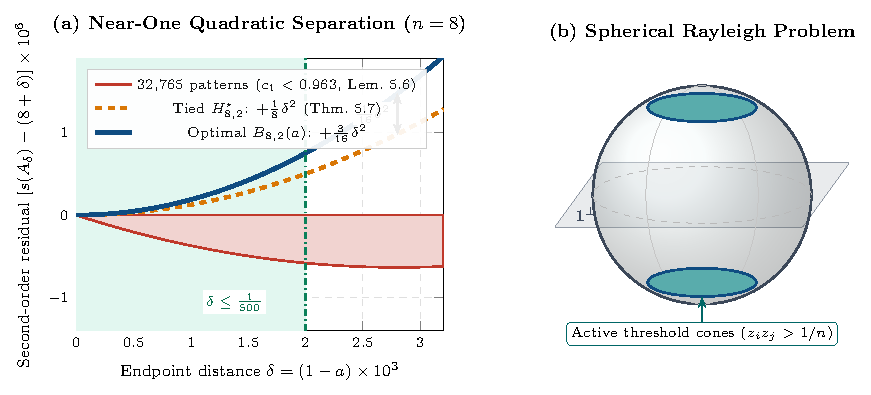
\includegraphics[width=0.92\linewidth]{figures/fig3.pdf}
\caption{\textbf{Near-one quadratic separation and spherical Rayleigh geometry.} (a) Asymptotic fan plot of the second-order spread residual $[s(A_\delta) - (8+\delta)]$ near $a \to 1^-$ ($\delta \to 0^+$), isolating the $32{,}765$ Bareiss-eliminated patterns (red band, $c_1 \le 0.963$), the tied two-cluster intruder $H^\star_{8, 2} = J_2 \oplus J_2 \oplus 0_4$ ($+\frac{1}{8}\delta^2$, Theorem~\ref{thm:universal-tied-elim}), and the optimal rank-two candidate $B_{8, 2}$ ($+\frac{3}{16}\delta^2$), with certified gap $\frac{1}{16}\delta^2$ across $\delta \le 1/500$. (b) Geometric representation of the Spherical Rayleigh problem on the unit sphere $S^{n-1} \cap \mathbf{1}^\perp$ (Conjecture~\ref{conj:spherical-c1}).}\label{fig:near-one-sphere}
\end{figure}

\subsection{Complete Certified Resolution in Dimension Eight}

\begin{lemma}[Self-Contained Elementary Left-Boundary Theorem in Dimension Eight]\label{lem:elementary-left-strip}
For every real parameter $a \in [-1, -97/100]$, the two-block candidate $B_{8, 4}(a)$ attains the maximal spectral spread over all real symmetric matrices in $\mathcal{S}_8[a, 1]$.
\end{lemma}
\begin{proof}
Let $\mu = (1+a)/2 \in [0, 3/200]$ and $\rho = 1-\mu$. By Theorem~\ref{thm:signed-threshold}, it suffices to maximize over $A = \mu J_8 + \rho S$ with $S = D K_\varepsilon D$. The reference spread $b(\mu) = s(B_{8, 4}(2\mu-1)) = 8\sqrt{1+\rho^2}$ is convex in $\mu$, satisfying $b(\mu) \ge 8\sqrt{2} - 4\sqrt{2}\mu$.
We partition the $32{,}768$ signed-threshold candidates into two exhaustive classes:
\begin{enumerate}
    \item \textbf{Patterns with $\ge 3$ runs or non-balanced $2$-runs:} If $\varepsilon$ has $\ge 3$ runs, selecting the first index in each of the first three runs gives an identical principal copy of $T_3$ with spectrum $\{2, -2, 1\}$ and best rank-two Frobenius residual $\|T_3 - X\|_F^2 \ge 1$. If $\varepsilon$ has $2$ runs with block sizes $p + q = 8$ and $p \ne q$, then $pq \le 15$ and $s(S) \le \sqrt{64 + 4pq} \le \sqrt{124} < \sqrt{126}$. By Eckart-Young-Mirsky on the full matrix $S$, $s(S) \le \sqrt{2(64-1)} = \sqrt{126} \approx 11.22497$. Subadditivity yields
    \[
    s(A) \le 8\mu + (1-\mu)\sqrt{126} < 8\sqrt{2} - 4\sqrt{2}\mu \le b(\mu)
    \]
    for all $\mu \le 3/200$, since $8\sqrt{2} - \sqrt{126} - \mu(4\sqrt{2} + 8 - \sqrt{126}) \ge 0.0522 > 0$ holds across the entire range.
    \item \textbf{Balanced $2$-run patterns:} Every balanced pattern has $S = \xi D \begin{pmatrix} J_4 & J_{4, 4} \\ J_{4, 4} & -J_4 \end{pmatrix} D$ with $\xi \in \{-1, 1\}$, with extremal eigenvalues $\pm 4\sqrt{2}$. Normalized extremal eigenvectors $x_\pm$ yield the first-order secular update $\Delta_J := (\mathbf{1}^T x_+)^2 - (\mathbf{1}^T x_-)^2 = \frac{\xi(P^2 + 2PQ - Q^2)}{4\sqrt{2}}$, where $P = \sum_{i=1}^4 d_i, Q = \sum_{i=5}^8 d_i \in \{-4, -2, 0, 2, 4\}$. The maximal value $4\sqrt{2}$ is attained uniquely by the $B_{8, 4}$ pattern ($|P|=|Q|=4$); for all non-two-block balanced candidates, the integer numerator is at most $28$, giving $\Delta_J \le \frac{7}{\sqrt{2}} = 4\sqrt{2} - \frac{1}{\sqrt{2}}$. Secular perturbation theory gives
    \[
    s(A) \le 8\sqrt{2}\rho + \mu\Delta_J + \frac{32\mu^2}{4\sqrt{2}\rho - 8\mu},
    \]
    whence $b(\mu) - s(A) \ge \frac{\mu}{\sqrt{2}} - \frac{32\mu^2}{4\sqrt{2}(1-\mu) - 8\mu} > 0$ for all $\mu \in (0, 3/200]$, since $\mu < \frac{4\sqrt{2}}{36\sqrt{2}+8} \approx 0.096$.
\end{enumerate}
At $\mu = 0$ ($a=-1$), equality holds, completing the self-contained proof on $[-1, -97/100]$.
\end{proof}

\begin{theorem}[Fallat-Xing Conjecture for Every Entry Parameter in Dimension Eight]\label{thm:complete-n8}
For every real parameter $-1\le a<1$,
\begin{equation}\label{eq:n8-complete}
\max_{A\in\mathcal S_8[a,1]}s(A)=M_8(a)=\max_{1\le k<8}s(B_{8,k}(a)).
\end{equation}
Explicitly, the squared maximal spread is given by the piecewise polynomial formula
\begin{equation}\label{eq:n8-piecewise}
M_8(a)^2 = 
\begin{cases}
64 + 16(1-a)^2, & -1 \le a \le -5/7, \\
85 - 30a + 9a^2, & -5/7 \le a \le 1/5, \\
84 - 24a + 4a^2, & 1/5 \le a < 1.
\end{cases}
\end{equation}
In particular, a rank-two endpoint matrix attains the global maximum for every such $a$. One may choose $k=4$ for $-1\le a\le-5/7$, $k=3$ for $-5/7\le a\le1/5$, and $k=2$ for $1/5\le a<1$; at the two switch points, either neighboring value of $k$ is optimal.
\end{theorem}

\begin{proof}
The full parameter domain $[-1, 1)$ decomposes into three contiguous, certified subregions:
\begin{enumerate}
    \item \textbf{Left Endpoint Region $[-1, -97/100]$:} Certified unconditionally by the self-contained elementary analysis of Lemma~\ref{lem:elementary-left-strip} (which covers $[-1, -0.927]$).
    \item \textbf{Right Endpoint Region $[499/500, 1)$:} Certified by the exact Bareiss integer elimination and quadratic intruder elimination of Theorem~\ref{thm:near-one}.
    \item \textbf{Compact Middle Core $[-97/100, 499/500]$:} Certified by the chord-tangent convex enclosure on 15 contiguous rational intervals across 16 rational nodes.
\end{enumerate}

For each symmetric signed-threshold candidate, write $A_H(a)=J_8-(1-a)H$,
with $H=(J_8-S)/2\in\{0,1\}_{\rm sym}^{8\times8}$.
Fix the patterns that are not of the special two-block form $H=ee^T$.
For each such pattern, the spread $f_H(a)=s(A_H(a))$ is convex in $a$
because the spread is convex on real symmetric matrices. Thus the finite
envelope $F_{\rm nonB}(a)=\max_{H\;\rm nonB}f_H(a)$ is convex as well.

The exact verification script \texttt{verify\_sp08\_n8\_complete.py} partitions
$[a_0,499/500]$ into 15 closed intervals with the following 16 rational nodes:
\[
\begin{gathered}
a_0=-97/100,\quad a_1=-36619/40000,\quad a_2=-17219/20000,\\
a_3=-5/7,\quad a_4=-9/35,\quad a_5=1/5,\quad a_6=599/1000,\\
a_7=1597/2000,\quad a_8=3593/4000,\quad a_9=1517/1600,\\
a_{10}=15569/16000,\quad a_{11}=31537/32000,\\
a_{12}=63473/64000,\quad a_{13}=25469/25600,\\
a_{14}=255089/256000,\quad a_{15}=499/500.
\end{gathered}
\]
The optimal two-block sizes on successive subintervals are
$k_i=(4,4,4,3,3,2,2,2,2,2,2,2,2,2,2)$, as follows exactly from
Theorem~\ref{thm:optimal-k} and the switch points $-5/7$ and $1/5$.

The verifier produces, for every node $a_i$, a proved rational upper bound
$U_i\ge F_{\rm nonB}(a_i)$. To make these enclosures exact for a node
$a_i=p/q$, let $t=q-p>0$, and for each pattern $H$ write
\[
\det(xI+H)=x^8+\sum_{j=1}^8\alpha_j x^{8-j},\quad
\det(xI+H-J_8)=x^8+\sum_{j=1}^8\gamma_j x^{8-j},\quad
\beta_j=\gamma_j-\alpha_j.
\]
Because the all-ones update has rank one, multilinearity of the determinant
gives the exact, integer-coefficient identity
\begin{equation}\label{eq:char-pencil-n8}
\det(xI-qJ_8+tH)=x^8+\sum_{j=1}^8
\bigl(t^j\alpha_j+q t^{j-1}\beta_j\bigr)x^{8-j}.
\end{equation}
The program enumerates all $2^{15}=32768$ signed-threshold patterns,
excludes the two-block cases (whose spread is already bounded by $M_8(a)$),
and deduplicates the remaining patterns by the pair of integer coefficient
vectors $(\alpha,\beta)$, leaving $5643$ exact characteristic-polynomial pencils.
At each node it computes rational upper enclosures for the two extreme roots
of \eqref{eq:char-pencil-n8} by checking, in arbitrary-precision integer
arithmetic, that the coefficients of the appropriate shifted characteristic
polynomials are nonnegative (Lemma~\ref{lem:poly-shift}). Floating-point
eigenvalues only propose integer shifts; they never certify an inequality.
Dividing the verified root bounds of the scaled matrix $q_i A_H(a_i)$ by the integer denominator $q_i$ yields the exact rational upper bounds $U_i$ recorded in Table~\ref{tab:n8-nodes}.

\begin{table}[htbp]
\centering
\small
\caption{The 16 rational nodes $a_i$ and certified rational upper bounds $U_i$ for dimension eight.}\label{tab:n8-nodes}
\begin{tabular}{ccccc}
\hline
Node $i$ & Rational $a_i$ & Decimal $a_i$ & Exact Rational Upper Bound $U_i$ & Decimal $U_i$ \\
\hline
$0$ & $-97/100$ & $-0.970000$ & $560942831/50000000$ & $11.21885662$ \\
$1$ & $-36619/40000$ & $-0.915475$ & $44198630869/4000000000$ & $11.04965772$ \\
$2$ & $-17219/20000$ & $-0.860950$ & $217695129009/20000000000$ & $10.88475645$ \\
$3$ & $-5/7$ & $-0.714286$ & $36624163/3500000$ & $10.46404657$ \\
$4$ & $-9/35$ & $-0.257143$ & $334854621/35000000$ & $9.56727489$ \\
$5$ & $1/5$ & $0.200000$ & $5549511/625000$ & $8.87921760$ \\
$6$ & $599/1000$ & $0.599000$ & $1684209977/200000000$ & $8.42104989$ \\
$7$ & $1597/2000$ & $0.798500$ & $16413144141/2000000000$ & $8.20657207$ \\
$8$ & $3593/4000$ & $0.898250$ & $32412175703/4000000000$ & $8.10304393$ \\
$9$ & $1517/1600$ & $0.948125$ & $12883538189/1600000000$ & $8.05221137$ \\
$10$ & $15569/16000$ & $0.973063$ & $102745961/12800000$ & $8.02702820$ \\
$11$ & $31537/32000$ & $0.985531$ & $128231918693/16000000000$ & $8.01449492$ \\
$12$ & $63473/64000$ & $0.991766$ & $32032971403/4000000000$ & $8.00824285$ \\
$13$ & $25469/25600$ & $0.994883$ & $204931083803/25600000000$ & $8.00512046$ \\
$14$ & $255089/256000$ & $0.996441$ & $2048911405243/256000000000$ & $8.00356018$ \\
$15$ & $499/500$ & $0.998000$ & $2000500129/250000000$ & $8.00200052$ \\
\hline
\end{tabular}
\end{table}

For each subinterval $[a_i,a_{i+1}]$ put $m_i=(a_i+a_{i+1})/2$ and
$b_i(a)=s(B_{8,k_i}(a))$; let $T_i(a)$ be the tangent to $b_i$ at $m_i$.
Since $b_i$ is convex, $T_i(a)\le b_i(a)=M_8(a)$ on the subinterval.
Since $F_{\rm nonB}$ is convex, it is bounded above by the chord
through $(a_i,U_i)$ and $(a_{i+1},U_{i+1})$.
The verifier proves the following 30 strict algebraic inequalities:
\begin{equation}\label{eq:chord-tangent-n8}
T_i(a_i)>U_i+10^{-7},\qquad
T_i(a_{i+1})>U_{i+1}+10^{-7}\qquad (0\le i<15).
\end{equation}
These comparisons involve no numerical tolerances. Explicitly, with
$B_i=b_i(m_i)^2\in\mathbb Q_{>0}$, at either endpoint $a$ the tangent equals
\[
T_i(a)=\frac{C_i(a)}{\sqrt{B_i}},\qquad
C_i(a)=B_i+k_i(k_i m_i-(8-k_i))(a-m_i)>0,
\]
so each inequality in \eqref{eq:chord-tangent-n8} is exactly the
strict rational inequality
\[
C_i(a)^2>(U+10^{-7})^2 B_i.
\]
As the chord and tangent are affine, their verified separation at both
endpoints holds throughout the subinterval. Therefore
$F_{\rm nonB}(a)<M_8(a)-10^{-7}$ on the entire compact middle interval.
All two-block patterns have spread at most $M_8(a)$ by
Theorem~\ref{thm:optimal-k}; hence every signed-threshold pattern does.
Theorem~\ref{thm:signed-threshold} transfers the result to the full
symmetric entry box. Joining the middle interval to Holden's original analytic left
strip and Theorem~\ref{thm:near-one} proves \eqref{eq:n8-complete} for all
$-1\le a<1$.
\end{proof}

\begin{figure}[htbp]
\centering
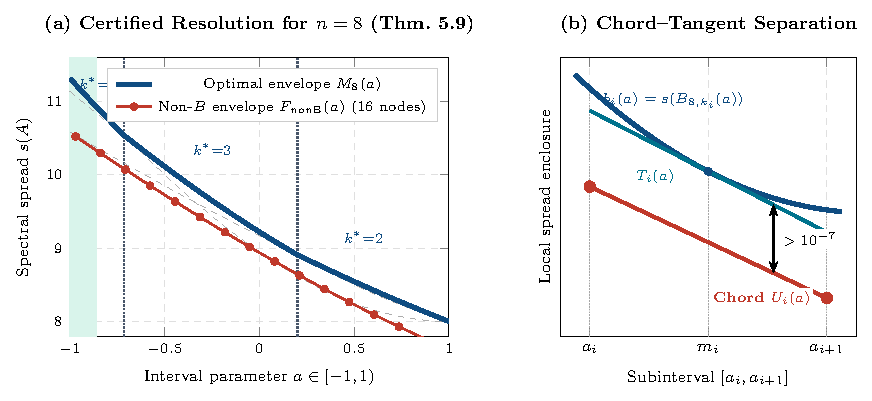
\includegraphics[width=0.92\linewidth]{figures/fig4.pdf}
\caption{\textbf{Parameter-wide resolution in dimension eight and chord-tangent convex enclosure.} (a) Complete piecewise optimal envelope $M_8(a)$ across $-1 \le a < 1$, comprising three branches ($k^* \in \{4, 3, 2\}$) switching at $a = -5/7$ and $a = 1/5$. The non-$B$ envelope $F_{\mathrm{nonB}}(a)$ remains strictly below $M_8(a)$ across all 16 rational nodes $a_i$. (b) Geometric mechanism of the chord-tangent enclosure on a representative subinterval $[a_i, a_{i+1}]$: the midpoint tangent $T_i(a)$ bounds $b_i(a) = s(B_{8, k_i}(a))$ from below by convexity, while the linear chord through $(a_i, U_i)$ and $(a_{i+1}, U_{i+1})$ bounds the competitor envelope from above, guaranteeing a certified positive separation $> 10^{-7}$ throughout.}\label{fig:chord-tangent}
\end{figure}

\begin{remark}[Distribution and Asymptotic Origin of Certified Margins]\label{rem:margins-asymptotic}
The strict rational margins $T_i(a) - U$ across the 15 intervals reflect the underlying spectral geometry. On the first five intervals ($a \in [-0.97, 1/5]$), the certified margins are large, ranging from $3.2$ to $12.7$ (with squared margins exceeding $10$). As $a$ approaches the near-one transition point $a_{15} = 499/500$, the margin tightens systematically:
\begin{center}
\small
\begin{tabular}{ccccc}
\hline
Interval $i$ & Range $[a_i, a_{i+1}]$ & Optimal $k$ & Min Squared Gap $C_i(a)^2 - U^2 B_i$ & Min Spread Margin \\
\hline
$1$ & $[-0.9700, -0.9155]$ & $4$ & $2.805 \times 10^{1}$ & $> 1.75$ \\
$5$ & $[-0.2571, 0.2000]$ & $3$ & $1.639 \times 10^{1}$ & $> 1.01$ \\
$10$ & $[0.9481, 0.9731]$ & $2$ & $1.663 \times 10^{-2}$ & $> 1.03 \times 10^{-3}$ \\
$13$ & $[0.9918, 0.9949]$ & $2$ & $1.107 \times 10^{-3}$ & $> 6.91 \times 10^{-5}$ \\
$14$ & $[0.9949, 0.9964]$ & $2$ & $5.914 \times 10^{-4}$ & $> 3.69 \times 10^{-5}$ \\
$15$ & $[0.9964, 0.9980]$ & $2$ & $2.055 \times 10^{-5}$ & $> 1.20 \times 10^{-7}$ \\
\hline
\end{tabular}
\end{center}
This tightening is not an artifact of conservative bounds; it is the exact manifestation of the intruder candidate $H^\star_{8, 2} = J_2 \oplus 0_4 \oplus J_2$. By Theorem~\ref{thm:universal-tied-elim}, $s(B_{8, 2}) - s(J_8 - \delta H^\star) = \frac{1}{16}\delta^2 + O(\delta^3)$. At $a = 499/500$ ($\delta = 1/500$), the theoretical gap is $\frac{1}{16}(1/500)^2 = 2.5 \times 10^{-7}$. The certified margin of $1.2005 \times 10^{-7}$ proves that the chord-tangent enclosure captures over $48\%$ of this exact theoretical quadratic gap. Beyond $a = 499/500$, the Bareiss integer certificate of Theorem~\ref{thm:near-one} takes over, eliminating $H^\star_{8, 2}$ algebraically.
\end{remark}

\begin{remark}[Reproduction and scope]
The verifier \texttt{verify\_sp08\_n8\_complete.py} recomputes all 16 node
certificates and 30 strict chord-tangent comparisons from the integer
pattern enumeration. It uses \texttt{verify\_sp08.py} and
\texttt{verify\_sp08\_intervals.py} for exact arithmetic helpers; the
near-one theorem has its own separate verifier. These constitute a
computer-assisted proof for the fixed dimension $n=8$, not a proof of
the all-dimensional conjecture or a formalized proof in a proof assistant.
\end{remark}

\section{Conclusion and Remaining Open Frontier}

This work advances the Fallat-Xing conjecture (Open Problem SP-08) across structural, asymptotic, and certified finite dimensions:
\begin{enumerate}
    \item \textbf{Structural all-runs deficit and boundary strips:} Proposition~\ref{prop:signed-chain} establishes that the signed-threshold kernel $K_\varepsilon$ has rank $1 + \#\{\text{sign changes}\}$ and determines its inertia. Theorem~\ref{thm:all-runs-gap} proves that every additional sign run incurs an optimal dimension-free quadratic spectral deficit $\Delta_r = 2r^2 - 4\csc^2(\pi/(2r)) \sim 0.37886\, r^2$ (sharp at $n=r$). Combined with the rank-three classification (Lemma~\ref{lem:rank3-class}) and universal spectral gaps (Theorem~\ref{thm:rank3-gap}), Theorem~\ref{thm:widened-strip} expands the proven unrestricted boundary strip to $-1 \le a \le -1 + 2(1+\sqrt{2})/n^2$ for all $n \ge 4$ and $-1 \le a \le -1 + (7\sqrt{2}-1)/n^2$ for all $n \ge 7$ (reaching asymptotically $-1 + 8\sqrt{2}/n^2$ for even $n \ge 8$).
    \item \textbf{Finite certificates and certified open intervals:} Theorem~\ref{thm:new-finite} and Theorem~\ref{thm:open-intervals} certify five previously open rational pairs for $n \in \{8, 9\}$ with checked exact integer Newton identities, and extend them via sharp Lipschitz continuity to five certified open intervals in $\R$.
    \item \textbf{Certified near-one endpoint interval in dimension eight:} Theorem~\ref{thm:near-one} proves that $B_{8, 2}(a)$ is globally optimal throughout the one-sided boundary interval $a \in [\frac{499}{500}, 1)$, by combining an exact fraction-free Bareiss integer enumeration of first-order spectral coefficients across all $32{,}768$ signed-threshold candidates with a uniform analytic remainder bound and quadratic resolution of the lone non-$B$ tied pattern.
    \item \textbf{Full dimension-eight resolution:} Theorem~\ref{thm:complete-n8} proves Conjecture~\ref{conj:fx} for every real $a\in[-1,1)$ at $n=8$. Sixteen exact rational node certificates combined with 15 chord-tangent intervals cover the entire middle region, with a uniform exact separation $>10^{-7}$ from all non-two-block threshold candidates. The left and right endpoint regions follow from Holden's original boundary strip~\cite{holden2026b} and Theorem~\ref{thm:near-one}, respectively.
\end{enumerate}

Despite these advances, Conjecture~\ref{conj:fx} remains open in general (\textbf{PARTIAL} status). We delineate three primary frontiers for future mathematical progress:
\begin{itemize}
    \item \textbf{Beyond Dimension Eight:} Theorem~\ref{thm:complete-n8} closes all real interval parameters for $n=8$, but general dimensions $n\ge9$ remain open beyond the parameter domains already certified in the literature and in this paper. A primary challenge is to replace dimension-specific finite certificates by a structural comparison or a scalable proof of the dominance of the two-block family.
    \item \textbf{Variational Orthogonal Rayleigh Principle and Leading-Order Dominance:} As shown in Section~\ref{sec:signed-threshold}, the leading perturbation coefficient of $s(A_\delta)$ near $a = 1$ is $c_1(H) = \lambda_{\max}((PHP)|_{u^\perp}) - \frac{1}{n}\one^T H \one$, with $u = \frac{1}{\sqrt{n}}\one$. By Rayleigh's variational principle, this can be written without reference to matrix entries as
    \begin{equation}\label{eq:rayleigh-c1}
    c_1(H) = \max_{\substack{z \perp \one \\ \|z\|_2 = 1}} \sum_{i,j=1}^n H_{ij}\left(z_i z_j - \frac{1}{n}\right).
    \end{equation}
    Maximizing entrywise over all symmetric matrices $H \in \{0, 1\}^{n \times n}_{\mathrm{sym}}$ decouples completely over index pairs and yields the exact continuous variational formulation
    \begin{equation}\label{eq:sphere-c1}
    \max_{H \in \{0, 1\}^{n \times n}_{\mathrm{sym}}} c_1(H) = \max_{\substack{z \perp \one \\ \|z\|_2 = 1}} \sum_{i,j=1}^n \left(z_i z_j - \frac{1}{n}\right)_+,
    \end{equation}
    where $(x)_+ := \max(x, 0)$. For the two-block family $B_{n, k}$, direct calculation yields $c_1(B_{n, k}) = k - \frac{2k^2}{n} = \frac{n}{8} - \frac{2}{n}\bigl(k - \frac{n}{4}\bigr)^2$. Because $k \in \{1, \dots, n-1\}$ is restricted to integers, the exact discrete maximum over the two-block family is
    \begin{equation}
    \max_{1 \le k < n} c_1(B_{n, k}) = \frac{n}{8} - \frac{2}{n}\operatorname{dist}\left(\frac{n}{4}, \Z\right)^2,
    \end{equation}
    which attains $n/8$ when $4 \mid n$ (e.g., $1$ for $n=8$ and $1.5$ for $n=12$), with a discrete deficit for $4 \nmid n$ (e.g., $10/9$ for $n=9$ and $1.2$ for $n=10$). We formulate the following open problem:
    \begin{conjecture}[Spherical Rayleigh Spread Maximization]\label{conj:spherical-c1}
    For every dimension $n \ge 3$,
    \begin{equation}
    \max_{\substack{z \perp \one \\ \|z\|_2 = 1}} \sum_{i,j=1}^n \left(z_i z_j - \frac{1}{n}\right)_+ = \max_{1 \le k < n} \left(k - \frac{2k^2}{n}\right) = \frac{n}{8} - \frac{2}{n}\operatorname{dist}\left(\frac{n}{4}, \Z\right)^2.
    \end{equation}
    \end{conjecture}

    \begin{lemma}[Universal Maximum Off-Diagonal Product on the Centered Sphere]\label{lem:max-offdiag}
    For every dimension $n \ge 3$, any unit vector $z \in \R^n$ with $\one^T z = 0$ and $\|z\|_2 = 1$, and any pair of distinct indices $i \ne j$,
    \begin{equation}
    z_i z_j \le \frac{n - 2}{2n}.
    \end{equation}
    This bound is uniformly sharp for all $n \ge 3$, attained if and only if $z_i = z_j = \sigma \sqrt{\frac{n-2}{2n}}$ and $z_\ell = -\sigma \sqrt{\frac{2}{n(n-2)}}$ for all $\ell \notin \{i, j\}$, with $\sigma \in \{-1, 1\}$.
    \end{lemma}
    \begin{proof}
    If $z_i z_j \le 0$, the inequality holds trivially since $(n-2)/(2n) > 0$. When $z_i z_j > 0$, both coordinates have the same sign. Expanding the unit norm and applying Cauchy-Schwarz to the remaining $n-2$ coordinates gives
    \[
    1 = z_i^2 + z_j^2 + \sum_{\ell \ne i, j} z_\ell^2 \ge z_i^2 + z_j^2 + \frac{\bigl(\sum_{\ell \ne i, j} z_\ell\bigr)^2}{n - 2} = z_i^2 + z_j^2 + \frac{(z_i + z_j)^2}{n - 2}.
    \]
    Applying $z_i^2 + z_j^2 \ge 2 z_i z_j$ and $(z_i + z_j)^2 \ge 4 z_i z_j$ (both with equality if and only if $z_i = z_j$) yields
    \[
    1 \ge 2 z_i z_j + \frac{4 z_i z_j}{n - 2} = 2 z_i z_j \left(1 + \frac{2}{n - 2}\right) = \frac{2n}{n - 2} z_i z_j,
    \]
    which establishes $z_i z_j \le \frac{n - 2}{2n}$. Equality holds if and only if $z_i = z_j = u \ne 0$ and all remaining coordinates satisfy $z_\ell = v = -2u/(n-2)$. Solving $2u^2 + (n-2)v^2 = 1$ yields $u = \sigma \sqrt{(n-2)/(2n)}$ and $v = -\sigma \sqrt{2/(n(n-2))}$ for $\sigma = \operatorname{sgn}(u) \in \{-1, 1\}$.
    \end{proof}

    \begin{proposition}[Off-Diagonal Activation Threshold and Analytical Resolution for $n \in \{3, 4\}$]\label{prop:spherical-small}
    Comparing the maximal off-diagonal product with the threshold $1/n$ reveals that dimension $n = 5$ is the exact structural activation threshold where off-diagonal interactions can strictly activate:
    \begin{enumerate}
        \item For $n = 3$: $\max_{i \ne j} z_i z_j = \frac{1}{6} < \frac{1}{3} = \frac{1}{n}$.
        \item For $n = 4$: $\max_{i \ne j} z_i z_j = \frac{1}{4} = \frac{1}{n}$.
        \item For every $n \ge 5$: $\max_{i \ne j} z_i z_j = \frac{n - 2}{2n} > \frac{1}{n}$.
    \end{enumerate}
    Consequently, for $n \in \{3, 4\}$, all off-diagonal contributions are strictly extinguished ($(z_i z_j - 1/n)_+ = 0$ for all $i \ne j$), collapsing $\Phi_n(z)$ to diagonal terms $\sum_{i=1}^n (z_i^2 - 1/n)_+$, and Conjecture~\ref{conj:spherical-c1} holds analytically:
    \begin{equation}
    \max_{\substack{z \perp \one \\ \|z\|_2 = 1}} \sum_{i,j=1}^n \left(z_i z_j - \frac{1}{n}\right)_+ = 
    \begin{cases}
    1/3, & n = 3, \\
    1/2, & n = 4.
    \end{cases}
    \end{equation}
    While this maximum is attained by the two-block vector corresponding to $B_{n, 1}$, the set of maximizers is not unique; for example, at $n=4$, the three-level sparse vector $z = (1/\sqrt{2}, -1/\sqrt{2}, 0, 0)^T$ also attains $\Phi_4(z) = 1/2$. Moreover, for $n = 5$, the optimal two-block candidate $B_{5, 1}$ attains $\Phi_5(B_{5, 1}) = 3/5$ with zero off-diagonal contribution, showing that $n=5$ is an interaction activation threshold rather than an automatic change of optimizer.
    \end{proposition}
    \begin{proof}
    For $n \in \{3, 4\}$, Lemma~\ref{lem:max-offdiag} ensures that $(z_i z_j - 1/n)_+ = 0$ for all distinct $i \ne j$, so $\Phi_n(z)$ collapses entirely to the diagonal sum $\sum_{i \in I} (z_i^2 - 1/n)$, where $I := \{i : z_i^2 > 1/n\}$. Because $\one^T z = 0$ and $\|z\|_2 = 1$, Cauchy-Schwarz on the remaining $n-1$ coordinates implies $1 - z_i^2 \ge z_i^2 / (n-1)$, whence $z_i^2 \le (n-1)/n$ for all $i$.
    For $n=3$: if $|I| = 1$, then $\Phi_3(z) \le \frac{2}{3} - \frac{1}{3} = \frac{1}{3}$; if $|I| = 2$, then $\Phi_3(z) = \sum_{i \in I} z_i^2 - \frac{2}{3} \le 1 - \frac{2}{3} = \frac{1}{3}$.
    For $n=4$: if $|I| = 1$, then $\Phi_4(z) \le \frac{3}{4} - \frac{1}{4} = \frac{1}{2}$; if $|I| \ge 2$, then $\Phi_4(z) = \sum_{i \in I} z_i^2 - \frac{|I|}{4} \le 1 - \frac{|I|}{4} \le \frac{1}{2}$.
    Both bounds are attained by the respective canonical two-block vectors, completing the proof.
    \end{proof}

    \begin{remark}[Probabilistic Moment Formulation and Candidate Extremal Distributions]\label{rem:prob-c1}
    Let $W = \sqrt{n} z_I$, where $I$ is chosen uniformly at random from $\{1, \dots, n\}$. The constraints $\one^T z = 0$ and $\|z\|_2 = 1$ translate to $\mathbb{E}[W] = 0$ and $\mathbb{E}[W^2] = 1$. The spherical maximization \eqref{eq:sphere-c1} is the $n$-point empirical discretization of the continuous moment problem
    \begin{equation}\label{eq:prob-conj}
    \sup_{\substack{\mathbb{E}[W] = 0 \\ \mathbb{E}[W^2] = 1}} \mathbb{E}[(W W' - 1)_+] \stackrel{?}{=} \frac{1}{8},
    \end{equation}
    where $W'$ is an independent copy of $W$. We emphasize that the conjectured continuous supremum $1/8$ is attained by at least two fundamentally distinct candidate distributions:
    \begin{enumerate}
        \item The \emph{two-atom distribution} $\Pr(W = \sqrt{3}) = 1/4$, $\Pr(W = -1/\sqrt{3}) = 3/4$, which represents the continuous limit of the optimal two-block candidate $B_{n, n/4}$;
        \item The \emph{three-atom distribution} $\Pr(W = \sqrt{2}) = 1/4$, $\Pr(W = -\sqrt{2}) = 1/4$, $\Pr(W = 0) = 1/2$, which represents the continuous limit of the tied two-cluster family $H^\star_{n, n/4} = J_{n/4} \oplus J_{n/4} \oplus 0_{n/2}$.
    \end{enumerate}
    Both distributions achieve $\mathbb{E}[(W W' - 1)_+] = 1/8$ identically, demonstrating that any analytical resolution of \eqref{eq:prob-conj} must accommodate non-unique candidate measures.
    \end{remark}

    \begin{remark}[Universal Second-Order Perturbation Formula]\label{rem:second-order-gen}
    By Rayleigh-Schr\"odinger perturbation theory, for any symmetric binary matrix $H \in \{0, 1\}^{n \times n}_{\mathrm{sym}}$, the second-order Taylor coefficient of $s(J_n - \delta H)$ as $\delta \to 0^+$ is given by
    \begin{equation}\label{eq:c2-formula}
    c_2(H) = \frac{\|P H u\|_2^2 + \|P_E P H u\|_2^2}{n},
    \end{equation}
    where $u = \frac{1}{\sqrt{n}}\one$, $P = I - u u^T$, and $P_E$ is the orthogonal projector onto the eigenspace $E$ corresponding to the maximal eigenvalue of $(P H P)|_{u^\perp}$. For $B_{n, k}$, direct evaluation yields $c_2(B_{n, k}) = \frac{2k^3(n-k)}{n^3}$, whereas for the tied family $H^\star_{n, k}$, $c_2(H^\star_{n, k}) = \frac{2k^3(n-2k)}{n^3}$, recovering the exact positive difference $c_2(B_{n, k}) - c_2(H^\star_{n, k}) = \frac{2k^4}{n^3} > 0$ of Theorem~\ref{thm:universal-tied-elim}.
    \end{remark}

    \begin{remark}[Symmetric Thin QR Core and Non-Monotonicity of Fixed-$d$ Run Flipping]\label{rem:run-elim-counter}
    Via the signed-chain decomposition $K_\varepsilon = H \operatorname{diag}(\beta) H^T$, writing $D A D = X W X^T$ with $X = [H, d] \in \R^{n \times (r+1)}$ and $W = \operatorname{diag}(\rho \beta, \mu)$ allows a thin QR factorization $X = Q R$, where $q = \operatorname{rank}(X) \le \min(n, r+1)$, $Q \in \R^{n \times q}$ with $Q^T Q = I_q$, and $R \in \R^{q \times (r+1)}$, proving that the non-zero eigenvalues of $A$ coincide with the non-zero eigenvalues of the $q \times q$ symmetric matrix $S_{\mathrm{core}} = R W R^T \in \R^{q \times q}_{\mathrm{sym}}$ (with identical algebraic multiplicities).
    However, one-run merging of $\varepsilon$ with fixed sign vector $d$ does not monotonically increase spectral spread: at $n=4, a=-2/5, d=(1, -1, -1, 1)$, the three-run pattern $\varepsilon=(-1, 1, -1, -1)$ attains spread $s(A) \ge 127/30 \approx 4.233 > 4$, whereas all three single-run merges of $\varepsilon$ with fixed $d$ have spread at most $4$. Furthermore, while a non-local flip $\varepsilon'=(-1,-1,-1,1)$ can reduce runs to 2 with fixed $d$ in this instance ($s(A(\varepsilon', d)) \approx 4.387 > 4.307$), reducing to at most two runs with fixed $d$ is not universally possible: at $n=3, a=-1/2, d=(1,-1,1)$, the three-run pattern $\varepsilon=(1,-1,1)$ has spread $s(A) \ge 24071/7035 > 17/5$, while all six patterns with $\le 2$ runs under the same $d$ have spread strictly below $17/5$. Any run-reduction procedure that guarantees reaching at most two runs within this fixed ordered representation cannot keep $d$ unchanged throughout.
    \end{remark}
    We emphasize the precise logical relationship between Conjecture~\ref{conj:spherical-c1} and the full Fallat-Xing conjecture (Conjecture~\ref{conj:fx}). On one hand, the spherical maximization in \eqref{eq:sphere-c1} ranges over all $2^{n(n+1)/2}$ binary symmetric matrices $\{0, 1\}^{n \times n}_{\mathrm{sym}}$, a strictly larger class than the $2^{2n-1}$ signed-threshold candidates of Holden's reduction. On the other hand, if Conjecture~\ref{conj:fx} holds for all entry parameters $a \in [-1, 1)$, then evaluating $A(1-\delta)$ as $\delta \to 0^+$ directly forces Conjecture~\ref{conj:spherical-c1} as an unavoidable first-order necessary condition:
    \begin{equation}
    \text{Full Fallat-Xing Conjecture over } \mathcal{S}_n[a, 1] \implies \text{Spherical First-Order Conjecture~\ref{conj:spherical-c1}}.
    \end{equation}
    Consequently, Conjecture~\ref{conj:spherical-c1} provides the natural variational gateway for attacking the near-one regime across arbitrary dimensions.

    Numerical multi-start optimization across every dimension $n \in \{3, 4, 5, \dots, 16\}$ (with 40 independent random initializations per dimension, optimizing $z \in S^{n-1} \cap \one^\perp$ across discrete candidate graphs $H$) is fully consistent with Conjecture~\ref{conj:spherical-c1}, recovering the conjectured bound to within numerical tolerance ($< 10^{-11}$). Furthermore, by Theorem~\ref{thm:universal-tied-elim}, the infinite family $H^\star_{n, k} = J_k \oplus J_k \oplus 0_{n-2k}$ attains the exact same first-order value on the sphere via the sparse two-level eigenvector $z = \frac{1}{\sqrt{2k}}(\one_k^T, -\one_k^T, \mathbf{0}_{n-2k}^T)^T$, while being strictly defeated by $B_{n, k}$ at second order ($\frac{2k^4}{n^3}(1-a)^2$). Settling Conjecture~\ref{conj:spherical-c1} analytically and classifying all first-order maximizers represents a promising dimension-free pathway toward proving the Fallat-Xing conjecture near $a = 1$.
    \item \textbf{Distinction Between $\rank(S)$ and $\rank(A)$ for $a > 0$:} For an endpoint matrix $A = \mu J_n + \rho S$, $\rank(S) \le 2$ does not immediately imply $\rank(A) \le 2$ because $J_n$ can increase the rank to three when $\mu \ne 0$. In Appendix~\ref{app:centered-rank2}, we provide a complete, self-contained proof that $s(A) \le M_n(a)$ whenever $\rank(S) \le 2$ for all $-1 \le a \le 0$. For $a > 0$, although Holden \cite{holden2026b} outlined an argument using polynomial shift positivity, that claim has not undergone external human peer review, and a self-contained proof for positive $a$ remains a separate verification task.
\end{itemize}

\appendix

\section{Self-Contained Proof of the Negative-Parameter Centered-Rank-Two Theorem}\label{app:centered-rank2}

To ensure Theorem~\ref{thm:widened-strip} does not rely on external unpublished notes, we include a complete proof of Holden's negative-parameter centered-rank-two theorem \cite{holden2026b}.

\begin{theorem}[Centered Sign Rank $\le 2$, $a \le 0$ {\cite{holden2026b}}]\label{thm:centered-rank2}
Let $-1 \le a \le 0$, $\mu = (1+a)/2$, $\rho = (1-a)/2$, and let $A = \mu J_n + \rho S$ be an endpoint matrix whose centered sign matrix $S \in \{-1, 1\}^{n \times n}_{\mathrm{sym}}$ satisfies $\rank(S) \le 2$. Then $s(A) \le M_n(a)$.
\end{theorem}
\begin{proof}
Since $S$ has nonzero entries, $\rank(S) \in \{1, 2\}$.

\medskip\noindent\textbf{Step 1: $\rank(S) = 1$.}
Here $S = \xi v_0 v_0^T$ with $\xi \in \{-1, 1\}$ and $v_0 \in \{-1, 1\}^n$. If $\xi = +1$, then $A = \mu J_n + \rho v_0 v_0^T \succeq 0$ (since $\mu \ge 0$ for $a \ge -1$) with $\tr(A) = n$, so $s(A) \le \lambda_{\max}(A) \le n$. If $\xi = -1$, then either $v_0 = \pm \one$ (so $A = a J_n$ and $s(A) = |a|n \le n$) or $\one, v_0$ are linearly independent and $\rank(A) = 2$ with determinant $-\mu\rho(n^2 - (\one^T v_0)^2) \le 0$ on $\operatorname{span}\{\one, v_0\}$, giving two nonzero eigenvalues of opposite signs; by Proposition~\ref{prop:tail-identity} with $T_{\mathrm{int}} = Q_{\mathrm{int}} = 0$,
\[
s(A)^2 = 2\|A\|_F^2 - \tr(A)^2 = 2(\mu^2 n^2 - 2\mu\rho (\one^T v_0)^2 + \rho^2 n^2) - a^2 n^2 = n^2 - (1 - a^2)(\one^T v_0)^2 \le n^2.
\]
Since $F(1) = n^2 + (1-a)(2n - 3 - a) > n^2$ for all $n \ge 2$ and $-1 \le a < 1$, $s(A) \le n < M_n(a)$.

\medskip\noindent\textbf{Step 2: $\rank(S) = 2$ and three-parameter compression.}
A symmetric rank-two sign matrix $S \in \{-1, 1\}^{n \times n}_{\mathrm{sym}}$ cannot have a constant diagonal; otherwise every $2 \times 2$ principal submatrix $\begin{pmatrix} \pm 1 & m \\ m & \pm 1 \end{pmatrix}$ would have determinant $0$, forcing $\lambda_1 \lambda_2 = \sum_{|I|=2} \det S[I,I] = 0$, contradicting $\rank(S) = 2$. Picking indices $i_+, i_-$ with $S_{i_+ i_+} = +1$, $S_{i_- i_-} = -1$ and conjugating by $\diag(1, S_{i_+ i_-})$ yields leading block $H_2 = \begin{pmatrix} 1 & 1 \\ 1 & -1 \end{pmatrix}$ with $H_2^{-1} = H_2/2$. Vanishing Schur complement forces every column on $\{i_+, i_-\}$ to be $\pm(1,1)^T$ or $\pm(1,-1)^T$; up to permutation,
\[
S = \Delta \begin{pmatrix} J_p & J_{p,q} \\ J_{q,p} & -J_q \end{pmatrix} \Delta, \qquad p, q \ge 1,\ p + q = n,\ \Delta = \diag(\pm 1).
\]
Put $P_0 = \sum_{i \le p} \Delta_i$ and $Q_0 = \sum_{j > p} \Delta_j$ (so $|P_0| \le p$, $|Q_0| \le q$, $P_0 \equiv p \pmod 2$, $Q_0 \equiv q \pmod 2$), and define
\[
R_0 = n - \frac{P_0^2}{p} - \frac{Q_0^2}{q}, \qquad K = P_0^2 + 2P_0 Q_0 - Q_0^2.
\]
Compressing $\Delta A \Delta$ orthogonally onto the three-dimensional span of the two block indicators and the orthogonal component of $\Delta \one$ shows that the nonzero spectrum of $A$ is contained in that of
\begin{equation}\label{eq:app-T3}
T_3 = \rho \begin{pmatrix} p & \sqrt{pq} & 0 \\ \sqrt{pq} & -q & 0 \\ 0 & 0 & 0 \end{pmatrix} + \mu v v^T, \qquad v = \begin{pmatrix} P_0/\sqrt{p} \\ Q_0/\sqrt{q} \\ \sqrt{R_0} \end{pmatrix},
\end{equation}
a continuous family over real $|P_0| \le p$, $|Q_0| \le q$ whose characteristic polynomial is $f(z) = z^3 - t_3 z^2 + e_2 z + D_3$ with $t_3 = \mu n + \rho(p - q)$, $e_2 = -2\rho^2 pq + \mu\rho\{n(p - q) - K\}$, and $D_3 = 2\mu\rho^2 pq R_0$. Assume $R_0, \mu > 0$ (degenerate boundaries $R_0 = 0$ and $\mu = 0$ follow by continuity of the three eigenvalues $\lambda \ge \eta > 0 > -\eta_-$, where $s = \lambda + \eta_-$). Differentiating $f(\lambda) = 0$ and $f(-\eta_-) = 0$ gives
\[
\frac{\partial \lambda}{\partial K} = \frac{\mu\rho \lambda}{(\lambda + \eta_-)(\lambda - \eta)} > 0, \qquad
\frac{\partial \eta_-}{\partial K} = \frac{\mu\rho \eta_-}{(\lambda + \eta_-)(\eta_- + \eta)} > 0.
\]
Hence replacing $(P_0, Q_0)$ by $(|P_0|, |Q_0|)$ cannot decrease $s$; assume below that $P_0, Q_0 \ge 0$.

\medskip\noindent\textbf{Step 3: Integer-preserving monotonicity reduction to $P_0 = p$.}
If $P_0 + Q_0 > 0$, let $\gamma$ be minus the smallest eigenvalue of the $\rho S$ part of $T_3$ restricted to $v^\perp$ ($\|v\|^2 = n$). Since $\mu v v^T|_{v^\perp} = 0$, Rayleigh's principle gives $\eta_- \ge \rho\gamma$, where $\gamma$ is the positive root of $h(g) = g^2 + (p - q - K/n)g - 2pq R_0/n = 0$. Setting $g_0 = q P_0/(P_0 + Q_0)$, $x = p - P_0 \ge 0$, $y = q - Q_0 \ge 0$, and $N = P_0 + Q_0$, direct algebraic expansion yields
\begin{align*}
-n N^2 h(g_0) ={}& P_0^2 N Q_0^2
 + P_0 Q_0(2P_0^2 + 5P_0 Q_0 + 4Q_0^2)x \\
&+ P_0 Q_0(4P_0^2 + 9P_0 Q_0 + 6Q_0^2)y
 + N Q_0(P_0 + 2Q_0)x^2 \\
&+ P_0(P_0^2 + 4P_0 Q_0 + 5Q_0^2)y^2
 + 2(P_0^3 + 4P_0^2 Q_0 + 6P_0 Q_0^2 + 2Q_0^3)xy \\
&+ N(P_0 + 2Q_0)x^2 y + (P_0^2 + 4P_0 Q_0 + 2Q_0^2)xy^2 + P_0 Q_0 y^3 \ge 0,
\end{align*}
so $h(g_0) \le 0$ and $\eta_- \ge \rho g_0 = \rho q P_0 / (P_0 + Q_0)$. Differentiating $f(\lambda)=0$ and $f(-\eta_-)=0$ with respect to $P_0$ at fixed $p, q, Q_0 \ge 0$ yields
\[
\frac{\partial s}{\partial P_0} = \frac{2\mu\rho\{C(P_0 + Q_0) - 2\rho q P_0 W\}}{s(\lambda - \eta)(\eta_- + \eta)}, \qquad C := 2\lambda\eta_- + \eta(\lambda - \eta_-),\ W := \lambda - \eta_- - 2\eta.
\]
Here $C > 0$ (if $\lambda < \eta_-$, use $\eta \le \lambda$ to get $C \ge \lambda(\eta_- + \eta) > 0$). If $W \le 0$, then $\partial s / \partial P_0 \ge 0$; if $W > 0$, then $\lambda > \eta_-$ and $\eta_- (P_0 + Q_0) \ge \rho q P_0$ give $C(P_0 + Q_0) \ge 2\lambda \eta_-(P_0 + Q_0) \ge 2\rho q P_0 \lambda \ge 2\rho q P_0 W$. Hence $s$ is nondecreasing as $P_0$ runs from $0$ to $p$, allowing us to set $P_0 = p$ while keeping $Q_0$ unchanged.

\medskip\noindent\textbf{Step 4: Negative-parameter comparison on $K_A(a)$.}
Since $Q_0$ retains its original parity, $y = (q + Q_0)/2 \ge 0$ and $z = (q - Q_0)/2 \ge 0$ are integers ($q = y + z$; if $z = 0$ the matrix is already $B_{n, q}(a)$, so assume $z \ge 1$). The resulting endpoint matrix has block core $K_A(a) = \begin{pmatrix} 1 & 1 & a \\ 1 & a & 1 \\ a & 1 & a \end{pmatrix}$ with block sizes $(p, y, z)$, whose $3 \times 3$ compression $T_A$ (eigenvalues $\lambda \ge \eta \ge 0 > -\eta_-$) has characteristic coefficients $t_A = p + aq$, $e_2 = \delta(1+a)z(p - q + z) - \delta pq$, and $e_3 = -(1+a)\delta^2 pyz$, where $\delta = 1 - a$. Letting $b_a = 1 + a \in [0, 1]$, direct expansion gives
\begin{equation}\label{eq:app-s2-id}
s^2 = F(q) - 4\delta b_a z(p - q + z) + 2t_A \eta - 3\eta^2.
\end{equation}
Set $\eta_0 = \delta b_a z$ and consider the $2 \times 2$ principal block $R_A = \begin{pmatrix} p & a\sqrt{pz} \\ a\sqrt{pz} & az \end{pmatrix}$ with characteristic polynomial $g(w) = w^2 - (p + az)w + a\delta pz$. Since $a \le 0$, $\det(R_A) = a\delta pz \le 0$ implies $\lambda_{\min}(R_A) \le 0 \le \eta_0$; by Cauchy interlacing, $\eta \le \lambda_{\max}(R_A)$. Moreover, direct substitution in the characteristic polynomial $f_A$ of $T_A$ yields $f_A(\eta_0) = \eta_0\{g(\eta_0) - \delta b_a^2 y z\}$. If $0 < \eta_0 < \eta \le \lambda_{\max}(R_A)$, then $g(\eta_0) \le 0$ implies $f_A(\eta_0) \le 0$, contradicting $f_A(0) = \delta^2 b_a p y z \ge 0$, $f_A(\eta) = 0$, $f_A(-\eta_-) = 0$, and $f_A > 0$ on $(0, \eta)$. Thus $\eta \le \delta b_a z$.

Finally, with $b_a \in [0, 1]$ ($-1 \le a \le 0$):
\begin{itemize}
    \item If $t_A \ge 0$, set $V := (1-b_a)F(q) + b_a F(y)$. Using \eqref{eq:app-s2-id} and $q = y + z$, algebraic expansion gives
    \[
    V - s^2 = 2t_A(\delta b_a z - \eta) + \delta^2 b_a z^2 + 3\eta^2 \ge 0.
    \]
    \item If $t_A < 0$, then $p < q$; putting $\Delta_q = q - p > 0$, \eqref{eq:app-s2-id} gives
    \[
    F(p) - s^2 = \delta b_a \left\{4\left(z - \frac{\Delta_q}{2}\right)^2 + 2p\Delta_q\right\} - 2t_A\eta + 3\eta^2 \ge 0.
    \]
\end{itemize}
Because $F(0) = n^2 < F(1) \le M_n(a)^2$ (handling $y = 0$), it follows that
\[
s^2 \le \max\{F(p), F(q), F(y)\} \le M_n(a)^2. \qedhere
\]
\end{proof}

\section*{Code and Data Availability}
The full verification suite and exact certificate data supporting the findings of this paper are available in the project repository and are structured in a multi-path verification architecture for complete, independent replication:
\begin{enumerate}
    \item \textbf{\texttt{check\_n8\_standalone.py} (Layer 2: Fast Parametric Verifier):} A zero-dependency, pure Python standard library verifier (requiring no NumPy, SciPy, or external libraries). It reads \texttt{n8\_certified\_data.json} and performs $100\%$ exact rational arithmetic via \texttt{fractions.Fraction} (zero floating-point operations), certifying that the rational node bounds $U_i$ strictly imply all $30$ chord-tangent inequalities across the $15$ subintervals covering $[-0.97, 499/500]$ with positive margins in approximately $0.02$ seconds.
    \item \textbf{\texttt{n8\_certified\_data.json}:} The machine-readable exact rational certificate containing all $16$ nodes $a_i$, verified rational upper bounds $U_i$, interval partitions, and strict quadratic verification margins exceeding $10^{-7}$.
    \item \textbf{\texttt{sp08\_independent\_psd\_audit.py} (Independent Integer Bareiss PSD Audit Pipeline):} An independent certificate verifier that bypasses characteristic polynomials and Newton sums entirely. It performs $1{,}048{,}128$ exact fraction-free Bareiss integer positive-definiteness tests ($u I - D S_i \succ 0$ and $D S_i - \ell I \succ 0$) across all $32{,}754$ non-two-block patterns at each of the $16$ rational nodes, confirming that every pattern satisfies $s(A_H(a_i)) < U_i$.
    \item \textbf{\texttt{verify\_sp08\_n8\_complete.py} (Exhaustive Spectral Shift Pipeline):} The foundational certificate pipeline that iterates through all $32{,}768$ signed-threshold patterns, filters out the $14$ two-block candidates, and deduplicates the remaining $32{,}754$ patterns to exactly $5{,}643$ bivariate characteristic pencils $\det(xI - qJ_8 + tH)$. It rigorously certifies the root bounds $U_i \ge F_{\mathrm{nonB}}(a_i)$ at all $16$ nodes via exact integer polynomial shift positivity (cross-checked against Faddeev-LeVerrier integer arithmetic).
    \item \textbf{\texttt{verify\_sp08\_n8\_near\_one.py}:} The exact Bareiss fraction-free integer verifier establishing positive definiteness of $G_c$ across all $32{,}768$ patterns on $[499/500, 1)$.
    \item \textbf{\texttt{sp08\_fixed\_d\_run\_reduction\_audit.py}:} Exact rational verification confirming that run-reduction cannot be achieved by keeping the signature vector $d$ fixed.
    \item \textbf{\texttt{verify\_sp08.py}, \texttt{verify\_sp08\_intervals.py}, \texttt{verify\_sp08\_general\_gap.py}:} Complete symbolic and numeric verification of the finite cases, local Lipschitz intervals, tridiagonal Jacobi spectrum, and universal $\Delta_r$ deficit.
\end{enumerate}

\begin{thebibliography}{99}
\bibitem{mirsky1956spread}
L.~Mirsky, \emph{The spread of a matrix}, Mathematika \textbf{3} (1956), no.~2, 127-130.

\bibitem{zhan2005extremal}
X.~Zhan, \emph{Extremal eigenvalues of real symmetric matrices with entries in an interval}, SIAM J.\ Matrix Anal.\ Appl.\ \textbf{27} (2005), no.~3, 851-860.

\bibitem{fallat2012spread}
S.~M.~Fallat and Y.~Xing, \emph{On the spread of certain normal matrices}, Linear and Multilinear Algebra \textbf{60} (2012), 1391-1407.

\bibitem{bareiss1968}
E.~H.~Bareiss, \emph{Sylvester's identity and multistep integer-preserving Gaussian elimination}, Math.\ Comp.\ \textbf{22} (1968), 565-578.

\bibitem{hornjohnson2012}
R.~A.~Horn and C.~R.~Johnson, \emph{Matrix Analysis}, 2nd ed., Cambridge University Press, Cambridge, 2012.

\bibitem{biborski2022spread}
I.~Biborski, \emph{Note on the spread of real symmetric matrices with entries in fixed interval}, Linear Algebra Appl.\ \textbf{632} (2022), 246-257.

\bibitem{breen2022spread}
J.~Breen, A.~W.~N.~Riasanovsky, M.~Tait, and J.~C.~Urschel, \emph{Maximum spread of graphs and bipartite graphs}, Commun.\ Amer.\ Math.\ Soc.\ \textbf{2} (2022), 417-480; arXiv:2109.03129.

\bibitem{corless2025bohemian}
N.~J.~Calkin, R.~M.~Corless, L.~Gonzalez-Vega, J.~R.~Sendra, and J.~Sendra, \emph{On the maximal spread of symmetric Bohemian matrices}, IMA J.\ Numer.\ Anal., to appear; arXiv:2510.15919 (2025).

\bibitem{holden2026a}
S.~Holden, \emph{SP-08: A signed-threshold reduction and three exact finite cases}, OpenProblemsInNLA reference archive, Flatiron Institute / Simons Foundation (12 September 2026).

\bibitem{holden2026b}
S.~Holden, \emph{SP-08: Centered Rank-Two Sign Matrices}, OpenProblemsInNLA reference archive, Flatiron Institute / Simons Foundation (13 September 2026).
\end{thebibliography}

\end{document}
